\section{轨迹目标、Surrogate 建模与概率性筛查}

本章接续上一章导出的逐 plume 观测量，说明这些离散、部分删失的图像测量如何被转换为可训练目标，并进一步用于不确定性感知 surrogate 和简化几何筛查。这样拆分的目的，是把“视频到观测量”的可审计图像流程与“观测量到预测器”的建模流程分开，使每一层的假设和边界更清楚。

短预喷进一步放大了测量轨迹与可训练目标之间的张力。
经典经验穿深定律在物理上仍有价值，但当观测窗口主要由喷射起始和喷射终止瞬态占据时，其适用性会下降。
第~2 章已建立的右删失问题在这里被作为目标构造约束，贯穿拟合、不确定性建模和蒸馏阶段。

\subsection{CDF 穿深轨迹的空间右删失审计}
\label{sec:cdf-spatial-censoring-audit-zh}
\newcommand{\scrNTotal}{24316}%
\newcommand{\scrNCensored}{9630}%
\newcommand{\scrRatePct}{39.6}%
\newcommand{\scrNaiveHoldGapMedianMm}{46}%

在构造拟合目标之前，需要先定量说明 CDF 穿深右删失问题的严重程度。这里的删失按空间上限定义，而不是按后续 surrogate 使用的 \(\SI{5}{ms}\) 训练窗口定义。对每个喷嘴族 \(n\)，审计脚本汇总多孔 Mie 工作流导出的全部正值 raw CDF penetration，并用 \(q=0.999\) 分位数估计该喷嘴族的视场上限 \(C_n\)。若一条 plume 的 raw 或 cleaned CDF 穿深轨迹达到 \(C_n-\epsilon_n\)，其中 \(\epsilon_n=\max(\SI{1}{mm},0.01C_n)\)，则将其标记为空间右删失。该审计由空间右删失审计脚本实现，比较 Mie 图像处理输出目录中的 raw Mie 输出与合成数据导出目录中的拟合目标（代码标识符见附录~\ref{app:implementation_mapping}）。

由此得到的标量诊断量为空间删失率（spatial censoring rate）：
\[
\mathrm{SCR}
=
\frac{1}{N}\sum_{i=1}^{N}
\mathbf{1}\!\left[
\max_t S_i^{\mathrm{raw/clean}}(t)
\ge C_{n(i)}-\epsilon_{n(i)}
\right],
\]
其中 \(n(i)\) 表示第 \(i\) 条轨迹所属的喷嘴族。

在 clean split 中，共有 \(\num{\scrNTotal}\) 条 CDF 穿深轨迹，其中 \(\num{\scrNCensored}\) 条满足空间右删失判据，对应空间删失率为 \(\scrRatePct\%\)。
喷嘴族视场上限的中位数为 \(\SI{92.52}{mm}\)。
在被删失的 clean 轨迹中，首次触及空间上限的中位时间为 \(\SI{1.76}{ms}\)，约位于 raw 正值观测时长的 \(44.4\%\)。
如果 naive 地把最后一个 cleaned CDF 穿深值一直保持到 \(\SI{5}{ms}\)，它相对 q1 接受拟合延拓的中位差距约为 \(\SI{\scrNaiveHoldGapMedianMm}{mm}\)；
即使把视场上限本身当作终端饱和值，相对 q1 延拓的中位差距仍为 \(\SI{43.96}{mm}\)。
这些差距不被解释为相对于宽视场真值的直接误差，因为本文没有匹配的宽视场测量；
它们用于量化若把触及空间上限的轨迹读作物理饱和，训练目标会继承多大的偏置。

\begin{figure}[t]
\centering
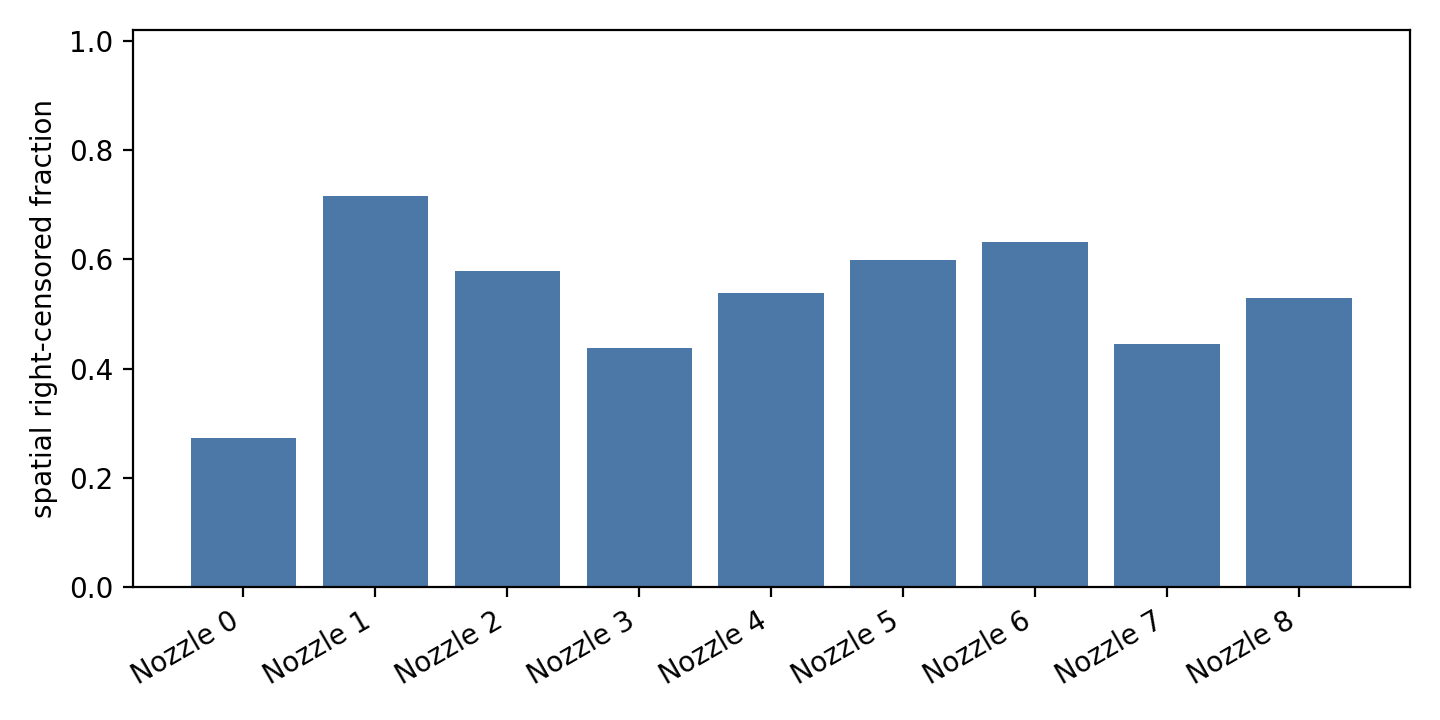
\includegraphics[width=0.88\linewidth]{images/fig_spatial_censoring_fraction_by_nozzle_clean.png}
\caption{clean CDF 穿深轨迹中按喷嘴族统计的空间右删失比例。
视场上限随喷嘴族而异，因为各族实验采用了不同的光学配置（相机距离、横向与纵向位置在喷嘴组间有所偏移），但同一族内的录像保持同一配置；喷嘴族因此作为视场上限的间接代理。
当 raw 或 cleaned CDF 穿深达到由 raw Mie 输出估计的喷嘴族视场上限时，该轨迹被计为空间右删失。
该审计表明，触及空间上限并非归档中的少数尾部案例：clean CDF 穿深轨迹总体约有 \(\scrRatePct\%\) 发生空间右删失。}
\label{fig:spatial-censoring-by-nozzle-clean-zh}
\end{figure}

\begin{table}[t]
\centering
\footnotesize
\begin{tabular}{@{}L{0.58\linewidth}L{0.34\linewidth}@{}}
\toprule
审计量 & clean CDF 穿深 split \\
\midrule
总轨迹数 & \(\num{\scrNTotal}\) \\
空间右删失轨迹数 & \(\num{\scrNCensored}\) (\(\scrRatePct\%\)) \\
喷嘴族视场上限中位数 & \(\SI{92.52}{mm}\) \\
被删失轨迹的首次触顶时间中位数 & \(\SI{1.76}{ms}\) \\
首次触顶位置占 raw 正值观测时长的中位比例 & \(44.4\%\) \\
naive-hold 相对 q1 延拓的中位差距 & \(\SI{\scrNaiveHoldGapMedianMm}{mm}\) \\
cap-saturation 相对 q1 延拓的中位差距 & \(\SI{43.96}{mm}\) \\
\bottomrule
\end{tabular}
\caption{clean CDF 穿深轨迹的空间删失审计摘要。最后两行将 naive 的删失目标构造与 \(\SI{5}{ms}\) 处的 q1 接受拟合延拓比较；这里将其作为目标偏置诊断，而不是相对于不可得宽视场真值的直接测量误差。}
\label{tab:spatial-censoring-audit-clean-zh}
\end{table}

该审计使建模后果变得明确。第~3 章交给本章的 raw CDF 穿深轨迹并不只是时间短或噪声大；其中相当一部分在 surrogate 目标时间范围之前已经触及喷嘴族空间上限。因此，降阶延拓、异方差教师模型以及后续 raw/KD 区制划分，是对已量化观测限制的回应，而不是额外的建模装饰。

\subsection{轨迹清洗与降阶拟合}

\subsubsection{轨迹清洗与时间对齐}

学习模型不直接在原始导出轨迹上训练。
清洗与拟合流程首先对它们进行清洗与Start of Injection (SOI)时间对齐。
对每个 plume，该流程先定位最早的有效穿深段，取SOI后的前两个非零样本点，对这些早期正值点做线性回归，并在斜率为正时用回归直线与 \(x\) 轴的截距作为亚帧级开启延迟估计。
如果 area 序列提供了更早的起始标记，则扫描从该帧锚定；
否则退回到首个正穿深帧。得到的原始延迟随后会在同一组 plume 内被裁剪限制到一个以中位数为中心的小窗口中，以避免单条异常 plume 把整组过度平移。

该延迟估计随后以两种耦合方式进入对齐过程。
穿深数组本身按最接近的整数帧数整体左移，而对齐后的时间轴则继续保留减去亚帧残差后的精确偏移。
因此，该处理在后续降阶拟合之前执行一次保留亚帧时序信息的 plume 起始配准。
完成对齐后，再移除不现实的突然跳跃，并通过一组基于规则的掩码标记低质量拟合。

\subsubsection{双分支候选模型}

Hiroyasu 和 Arai 将柴油喷雾穿深分为破碎前（\(\sqrt{t}\) 为主）与破碎后（\(t^{1/4}\) 为主）两个阶段\cite{HiroyasuArai1990}，
本节的双分支候选模型即以此为出发点。
在其基础上做两处适应：以可微 sigmoid 门替代刚性阶梯切换，从而获得光滑可微的拟合曲线；
同时使拟合不依赖除穿深观测值之外的任何外部物理量，令每条轨迹均可独立拟合。
此外，后续关于起始注入瞬态的研究表明，短注入难以用单一刚性经验表达式准确覆盖整条轨迹\cite{ZhouLiYi2021}——
这在本文中尤其突出，因为当前实验采用预喷柴油注入，其近 SOI 段短暂、高度瞬态且信噪比相对较低。

每个接受的轨迹随后用平滑的双分支模型拟合，
\[
S(t)=\left(1-w(t)\right)k_{\mathrm{sqrt}}\sqrt{t}
+w(t)k_{\mathrm{quarter}}t^{1/4},
\qquad
w(t)=\sigma\!\left(\frac{t-t_0}{s}\right),
\]
其中\(k_{\mathrm{sqrt}}\)、\(k_{\mathrm{quarter}}\)、\(t_0\)和\(s\)在对数空间中优化。具体来说，拟合问题表述为稳健的非线性最小二乘估计，
\[
\min_{\theta}
\sum_i \rho_\delta\!\left(S(t_i;\theta)-y_i\right),
\qquad
\theta=
\left[\log k_{\mathrm{sqrt}},\log k_{\mathrm{quarter}},\log t_0,\log s\right],
\]
使用Huber惩罚
\[
\rho_\delta(r)=
\begin{cases}
\tfrac{1}{2}r^2, & |r|\le \delta,\\
\delta\left(|r|-\tfrac{1}{2}\delta\right), & |r|>\delta.
\end{cases}
\]
其中 \(r = S(t_i;\theta)-y_i\) 为拟合残差，而 \(\delta\) 为误差惩罚从平方过渡到绝对值的阈值。该目标以信赖域非线性最小二乘法求解，取 \(\delta=1\)，
对数参数化保持拟合增益和转换尺度为正\cite{Huber1964,NocedalWright2006}。


因此，该模型应被理解为时间参数化而不是显式物理定律。其目的是双重的：
提供在EOI之外的可信外推，下游代理需要稳定目标；以及在SOI附近提供可接受的插值，其中相对误差较大，图像轨迹单独难以约束早期时间物理。
Sigmoid门在两个经验分支之间创建可微过渡，保持拟合曲线的平滑性，使其更兼容后续神经网络阶段。
换句话说，早期瞬态物理没有被强制进入刚性封闭形式定律；它们只是被足够好地近似，以便后续网络可以从完整的工况点输入中学习剩余的条件依赖行为。

当将拟合与喷雾文献中的扩展EOI表达式进行比较时，这种解释变得更加清晰。
Zhou等人报告的EOI后模型区分了全局注入时钟\(t\)和延迟时钟\((t-t_i)\)，因为后期穿深分支只有在结束注入动力学传播到下游后才激活\cite{ZhouLiLaiWei2019}。当前管线对这一延迟采用两层处理。首先，预处理阶段利用上文所述的早期线性外推，为每条 plume 估计一个起始延迟，并把观测序列平移到共同的 \(t\approx 0\) 参考上。其次，降阶拟合本身仍然没有把延迟时钟显式写进参数化分支，而是使用
\[
w(t)=\sigma\!\left(\frac{t-t_0}{s}\right)
\]
在学习的转换时间\(t_0\)之前抑制四分之一根分支，然后允许\(t^{1/4}\)项在该转换后主导。
这是一种工程重新参数化：
在有限观测窗口中，延迟第四根分支通常可以用一个门控未移位第四根分支很好地表示，调整幅度和转换位置，
特别是当该分支的早期部分通过\(1-w(t)\)或\(w(t)\)在零附近被强烈衰减时。
从这个意义上说，延迟物理时钟被吸收进学习的切换参数\((t_0,s)\)和分支幅度中，而不是作为固定已知常数强加。

因此，这一工程处理对本文目标是合理的，但边界需要明确：
该拟合用于压缩噪声轨迹，而不是作为最终机理喷雾定律；
它保持曲线可微以供后续学习，并把工况依赖性留给神经网络，而不是把每个物理效应强加进封闭形式拟合中。
这个解释应被理解为受经验穿深理论启发的降阶 surrogate，而不是证明移位时间物理已经消失。下文的四分之一根消融直接给出这一比较。

\subsubsection{四分之一根主导性与 q1 生产模型的选定}

若 \(k_{\mathrm{sqrt}}\) 在实践中几乎为零，那么保留该自由度不仅多余，还可能在困难轨迹上适得其反。对全部接受拟合的定量核查直接证实了前一点；下文的消融实验则证实了后一点。

对极坐标二值穿深归档中全部 \(14{,}563\) 个接受的 plume 拟合进行直接定量核查，可以更精确地确认这一点。
在拟合转换时刻 \(t_0\)，两条分支的幅值分别为 \(k_{1/4}\cdot t_0^{1/4}\)（四分之一根分支）和 \(k_{\mathrm{sqrt}}\cdot t_0^{1/2}\)（平方根分支）；
两者之比定义为
\[
r = \frac{k_{\mathrm{sqrt}}\cdot t_0^{1/4}}{k_{1/4}}.
\]
在所有接受的拟合样本中，该比值的中位数为 \(r_{\mathrm{med}}=2.9\times10^{-9}\)，四分位距为 \([9.0\times10^{-10},\;1.1\times10^{-8}]\)。
\(99.8\%\) 的样本满足 \(r<0.5\)，\(100\%\) 满足 \(r<1\)。
以绝对幅值表达：四分之一根分支在 \(t_0\) 时刻的中位贡献为 \(\SI{69.2}{mm}\)，
而平方根分支的中位贡献仅为 \(2.0\times10^{-7}\,\si{mm}\)，相差约八个数量级。
图~\ref{fig:ksqrt-ratio}展示了 \(\log_{10}(r)\) 的完整分布（面板~a）及四分之一根分支幅值分布（面板~b）。
在实践中，对于该归档中的每一个成功拟合，平方根项在转换时刻的贡献均可忽略不计，成功拟合实际上完全退化为以四分之一根为主导的曲线。
对本文的预期用途而言，这是可以接受的：物理驱动量会在后续直接输入神经网络，而拟合本身则保持自适应且物理负担较轻。

\begin{figure}[t]
\centering
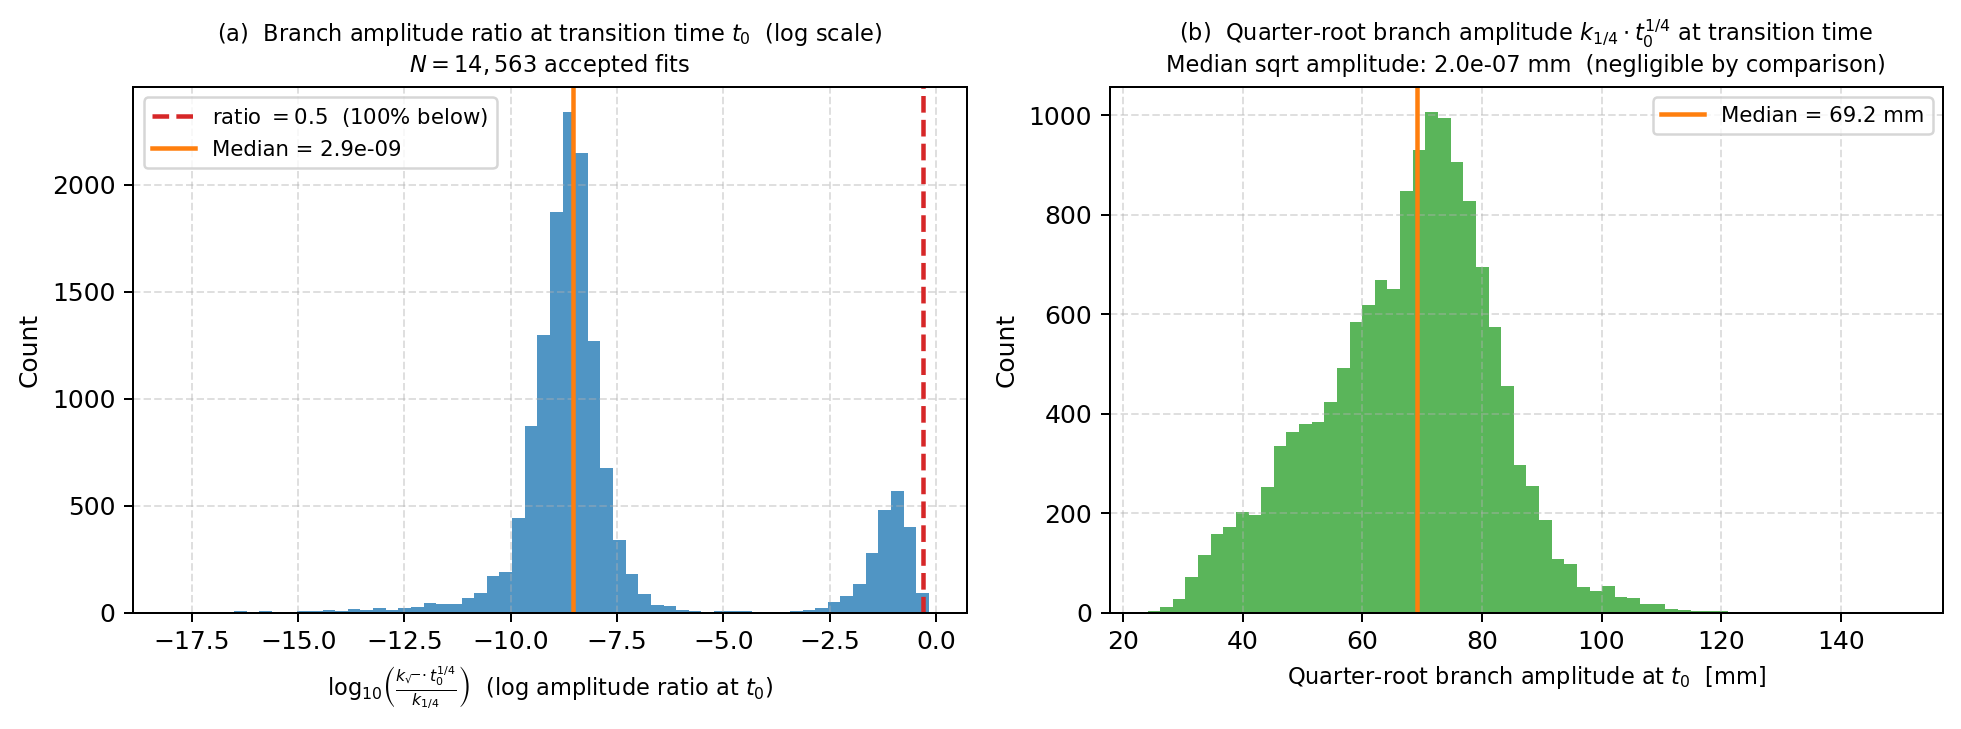
\includegraphics[width=0.96\linewidth]{images/ksqrt_ratio_distribution.png}
\caption{对 \(14{,}563\) 个接受的 plume 拟合（clean-fit 归档，极坐标二值穿深 数据源）中平方根分支权重的定量评估。
(a)~拟合转换时刻处分支幅值比 \(r=k_{\mathrm{sqrt}}\cdot t_0^{1/4}/k_{1/4}\) 的对数尺度分布；
红色虚线标注 \(r=0.5\)，99.8\% 的样本低于该阈值。
(b)~四分之一根分支幅值分布，中位值 \SI{69.2}{mm}，约为平方根分支中位幅值的八个数量级，确认几乎所有接受的拟合均以四分之一根为主导。}
\label{fig:ksqrt-ratio}
\end{figure}

这一观察直接引出一个结构消融：
如果成功的拟合本就收敛为以四分之一根为主导的曲线，那么残余的 \(k_{\mathrm{sqrt}}\) 自由度在困难轨迹上可能成为一个破坏性因素。
具体而言，当求解器无法在短截或噪声较大的轨迹上找到约束良好的最小值时，
无约束的 \(\sqrt{t}\) 项可能在优化过程中膨胀，将远时间外推驱向物理上不合理的数值，导致掩码流水线拒绝该序列，
尽管单独使用四分之一根分量本可以对其进行充分拟合。

单分支降阶模型（简称 q1，取自 quarter-root 单分支）将两区制混合替换为单一 sigmoid 门控四分之一根分支，消除了上述风险：
\[
S_{q1}(t) = \sigma\!\left(\frac{t-t_0}{s}\right)\,k_{1/4}\,t^{1/4},
\]
参数数量从四个缩减为三个：\([\log k_{1/4},\,\log t_0,\,\log s]\)。同时为 q1 并行构建了等效掩码流水线：在 \(t_{\mathrm{far}}=\SI{5}{ms}\) 处评估拟合曲线并与相同的物理合理窗口 \([18,\,300]\,\si{mm}\) 对比；应用相同的 \(t_0 < \SI{0.8}{ms}\) 和 \(s < \SI{1}{ms}\) 参数边界；并对 \(t_0\)、RMSE 和 cost-per-point 计算相同的分组稳健-\(z\) 异常值分数。当一条序列通过完整掩码流水线且满足 \(\mathrm{RMSE} < \SI{3}{mm}\) 时，即被计为拟合成功，使得两个模型的成功判据对称、可直接比较。

在九喷嘴 CDF 穿深数据集的全部 \(23{,}495\) 条序列中（已过滤掉少于十个有效帧的序列），四参数候选模型的成功率为 \(61.3\%\)，而 q1 模型的成功率为 \(90.0\%\)——绝对提升 28.6 个百分点，且无任何单个喷嘴出现退步。在两个模型均通过的干净子集上，四参数候选模型的 RMSE 中位数为 \(\SI{1.23}{mm}\)，q1 为 \(\SI{1.27}{mm}\)，证实去除 \(k_{\mathrm{sqrt}}\) 对表现良好的数据不造成损失。
而在被标记子集上，对比更为鲜明：RMSE 中位数从 \(\SI{8.12}{mm}\) 降至 \(\SI{1.08}{mm}\)，降幅约 \(7.5\times\)。
提升幅度：Nozzle 0 提升 37.6 个百分点，Nozzle~7 提升 28.7 个百分点
——减速阶段使 \(t^{1/4}\) 形式成为主导描述符、同时令 \(\sqrt{t}\) 分支在物理上失去意义的工况。

基于这一消融，q1 已被提升为生产拟合目标，后续 Stage~1、Stage~2 与 Stage~3 使用的都是 q1 导出的平滑目标，而不是继续把四参数候选模型作为训练标签。
四参数结果在本文中保留为结构诊断和历史基线，用于说明为什么需要降阶。
该拟合的实际目的，是把带噪 plume 轨迹压缩为平滑、可微且适合训练的目标，同时保留数据集中的异方差变化供后续学习阶段使用。

\subsubsection{q1 诊断：标度回归、残差结构与可辨识性}

\textbf{经验标度核查。} 对 \(24{,}316\) 个被接受的 q1 拟合做后处理标度回归，可以与经典穿深理论做一次合理性比对。
以最小二乘拟合 \(\log k_{1/4} = a\,\log\Delta P + b\,\log\rho_a + c\,\log d_n + \text{const}\)，
得到的指数为 \(a\approx 0.52\)、\(b\approx -0.23\)、\(c\approx 0.26\)，\(R^2\approx 0.27\)。
其中 \(\rho_a\) 指数与 Hiroyasu--Arai 破碎后形式 \(S\propto\Delta P^{1/4}\rho_a^{-1/4}(d_n t)^{1/2}\) 高度一致，
几乎精确匹配 \(-1/4\)。注入压力指数（\(a\approx 0.52\)）比 H--A 值 \(1/4\) 明显更陡，确切原因尚不清楚：
可能与 \(t^{1/4}\) 分支主要捕捉减速工况而非 H--A 所适用的自由射流阶段有关，也可能部分源于数据集的条件覆盖范围或拟合模型的函数形式，而非单一的物理机制。
喷孔直径指数（\(c\approx 0.26\)）明显低于经典值 \(1/2\)，可能反映了实验数据集中喷孔直径与其他工况变量之间的共线性。
门控参数 \(t_0\) 与 \(s\) 的回归 \(R^2\) 显著较低（\(0.17\) 与 \(0.14\)），这在意料之中：sigmoid 切换时刻不是 H--A 理论直接预测的物理量，它在数据预对齐之后吸收了剩余的起始延迟变异。
作为交叉验证，对原始离散穿深点按 0.1~ms 分桶做 \(\log S\) 的 log-log 回归，在中段（\(0.35\)--\(0.75\)~ms）得到 \(R^2\approx 0.47\)--\(0.51\)，表明三个物理变量在采样密集的时间窗口内确实能解释相当比例的穿深散点方差。\(k_{1/4}\) 回归所得 \(R^2\approx 0.27\) 偏低，主要反映该参数需对整段轨迹（含起始噪声和喷后截断段）积分，而非拟合失效；气室压力指数（\(\approx-0.25\)）及 \(\Delta P\) 指数（中段约 \(0.44\)--\(0.65\)，介于 Bernoulli 值 \(0.5\) 与 H--A 值 \(0.25\) 之间）在两种分析中保持一致。

\begin{figure}[t]
\centering
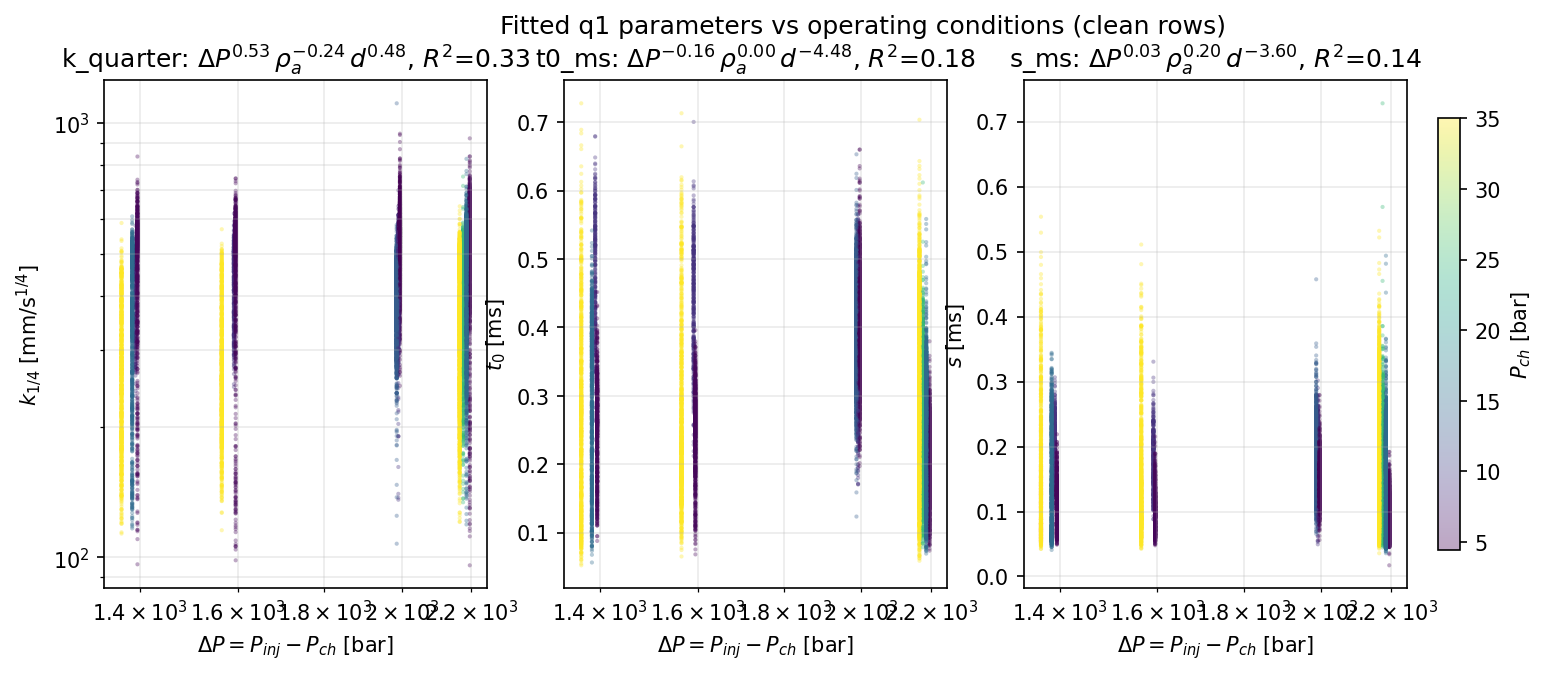
\includegraphics[width=0.96\linewidth]{images/fig_q1_param_scaling.png}
\caption{q1 生产参数 \((k_{1/4},t_0,s)\) 对 \(\Delta P=P_{\mathrm{inj}}-P_{\mathrm{ch}}\) 的经验标度，以腔压 \(P_{\mathrm{ch}}\) 着色。各子图标题给出了回归 \(\log y = a\log\Delta P + b\log\rho_a + c\log d_n + \text{const}\) 的拟合指数与 \(R^2\)。\(k_{1/4}\) 子图显示 \(\rho_a^{-0.23}\) 与 Hiroyasu--Arai 的 \(-1/4\) 预测高度吻合，而直径指数（\(d_n^{0.26}\)）明显低于经典值 \(1/2\)；门控参数则无法用同一组无量纲群很好地解释。}
\label{fig:q1-param-scaling}
\end{figure}

\textbf{残差结构与异方差性。} 对每条干净拟合在每个观测帧重建残差 \(\hat S(t)-y(t)\)，再以 \(\Delta t=\SI{0.1}{ms}\) 为时间分箱，可以得到图~\ref{fig:q1-residual-structure} 中的经验包络。该诊断揭示出两个截然不同的区段。在中段窗口 \(t\in[0.3, 1.0]\,\si{ms}\) 内，残差中位数始终保持在 \(\SI{0.4}{mm}\) 以下，稳健离散度 \(\sigma_{\mathrm{robust}}(t)=1.4826\,\mathrm{MAD}(t)\) 在 \(t=\SI{1.0}{ms}\) 附近达到最小值 \(\sim\SI{0.60}{mm}\)，确认 q1 在采样最充分的轨迹中段基本无偏且离散度较小。然而两端均出现残差膨胀：第一时间分箱（\(t=\SI{0.05}{ms}\)）携带 \(\sim\SI{+1.7}{mm}\) 的正偏，\(\sigma_{\mathrm{robust}}\approx\SI{1.8}{mm}\)，源于起始延迟对齐误差及 \(t_0\) 附近 sigmoid 门陡峭过渡；晚段尾部（\(t=\SI{1.55}{ms}\)）则携带 \(\sim\SI{-1.6}{mm}\) 的负偏，\(\sigma_{\mathrm{robust}}\approx\SI{0.7}{mm}\)，源于存活样本的右删失（每分箱样本数从 \(t=\SI{0.15}{ms}\) 处的 \(\sim 65{,}000\) 帧崩溃到 \(t=\SI{1.55}{ms}\) 处不足 \(200\)）。包络因此呈 U 形，而非单调增长；但对于代理模型栈而言，定性结论不变：残差尺度强烈依赖于时间，固定方差损失不再适用，Stage~2 必须学习输入相关的 \(\sigma\)，而不是单一标量。Stage-1 确定性基线捕捉的是该诊断所揭示的\emph{条件均值}，而\emph{条件离散度}（包括其边界膨胀）必须由 Stage~2 来解释。

\begin{figure}[t]
\centering
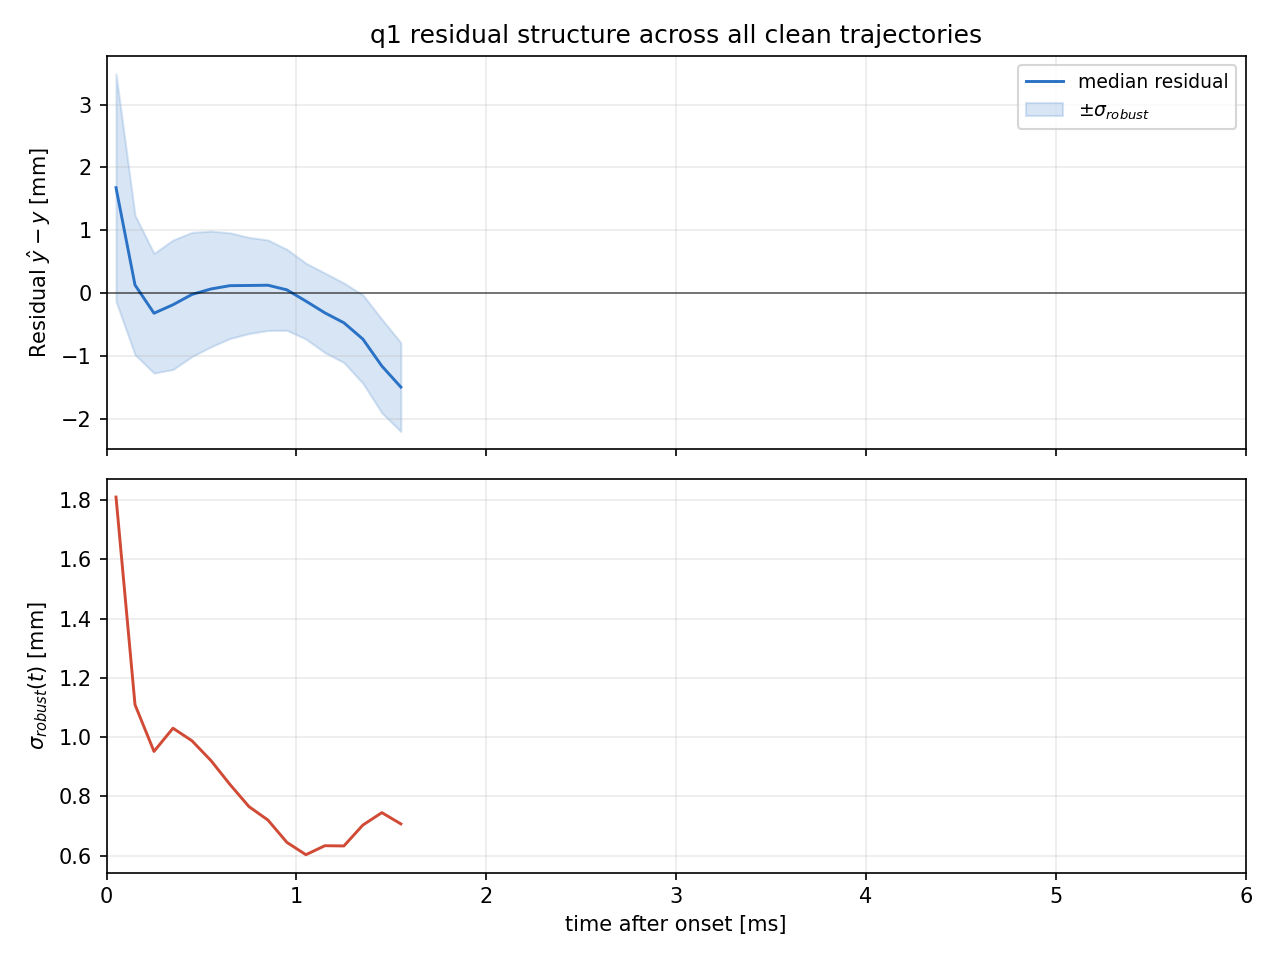
\includegraphics[width=0.92\linewidth]{images/fig_q1_residual_structure.png}
\caption{q1 生产拟合在全部 \(24{,}316\) 条干净轨迹上聚合得到的残差结构。上图：每个时间分箱的中位残差，阴影为 \(\pm\sigma_{\mathrm{robust}}\)；下图：稳健标准差 \(\sigma_{\mathrm{robust}}(t)=1.4826\,\mathrm{MAD}(t)\) 呈 U 形包络——起始延迟对齐噪声将第一分箱抬升至 \(\sim\SI{1.8}{mm}\)，中段在 \(t=\SI{1.0}{ms}\) 附近达到最小 \(\sim\SI{0.60}{mm}\)，晚段尾部因存活样本右删失而再次膨胀。\(\sigma(t)\) 的非恒定性正是 Stage-2 NLL 损失采用输入相关方差的动机所在。}
\label{fig:q1-residual-structure}
\end{figure}

\textbf{参数可辨识性。} 第三项诊断从 SciPy 返回的 trust-region Jacobian \(J\) 估计渐近参数协方差 \(\Sigma\approx (J^TJ)^{-1}\hat\sigma^2\)，并在所有干净拟合上汇总两两相关系数。中位相关系数为 \(\overline{\mathrm{corr}}(\log k_{1/4},\log s)\approx 0.76\)、\(\overline{\mathrm{corr}}(\log k_{1/4},\log t_0)\approx 0.56\)、\(\overline{\mathrm{corr}}(\log t_0,\log s)\approx 0.21\)。这些相关系数都偏强：q1 的三个参数并非彼此独立的物理把手，而是一个三维耦合的平滑面，存在显著的软冗余。这正是可微 sigmoid 门相对于 H--A 刚性分阶段断点所付出的代价，也解释了为什么上文标度回归中两个门控参数难以用同一无量纲群解释——数据只能整体约束这个三维曲面，而无法分别约束每一个参数。这一观察直接影响了下游设计选择：第~4.4 节中的代理模型被训练去复现整条评估曲线，而不是直接预测参数三元组本身，因此参数耦合不会传播进训练后网络的输入--输出映射中。

\begin{figure}[t]
\centering
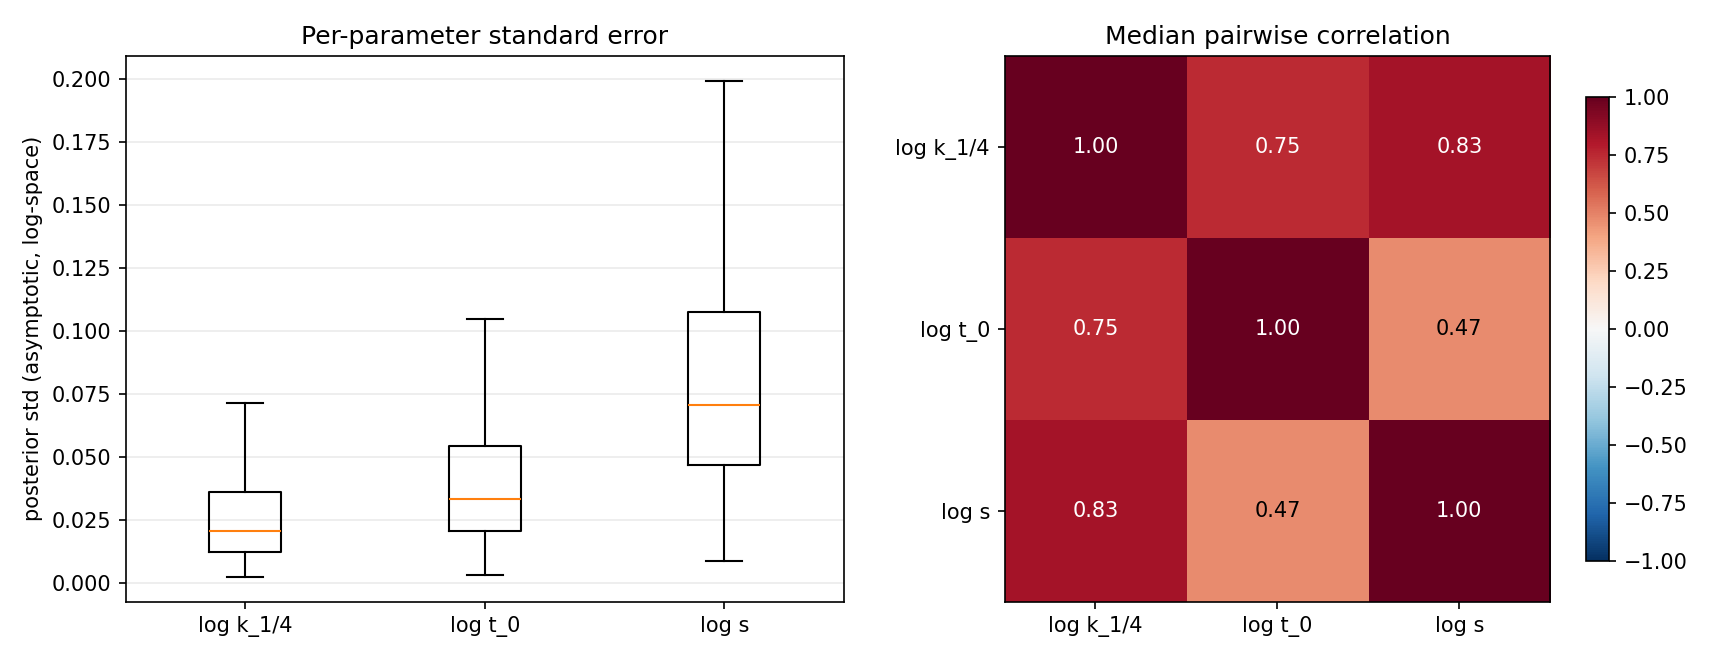
\includegraphics[width=0.96\linewidth]{images/fig_q1_identifiability.png}
\caption{q1 生产模型的逐拟合可辨识性诊断。左：\(\log k_{1/4}\)、\(\log t_0\)、\(\log s\) 渐近标准误差的分布（为可读性裁剪到 99\% 分位数）。右：\((J^TJ)^{-1}\) 给出的中位两两相关矩阵；非对角项 \(\sim 0.56\) 与 \(\sim 0.76\) 量化了分支幅度与 sigmoid 门之间的软冗余。}
\label{fig:q1-identifiability}
\end{figure}

表~\ref{tab:q1-fit-diagnostics-summary} 把上面四项诊断的关键数字汇总到一处，便于后文交叉引用。所有数值均由生产归档直接计算得到。

\begin{table}[t]
\centering
\caption{q1 拟合质量诊断在 \(24{,}316\) 条干净拟合与 \(703{,}592\) 帧观测上的统计汇总。}
\label{tab:q1-fit-diagnostics-summary}
\small
\begin{tabular}{p{0.30\linewidth} p{0.40\linewidth} p{0.22\linewidth}}
\toprule
\textbf{诊断项} & \textbf{统计量} & \textbf{数值} \\
\midrule
工况分组 RMSE & (nozzle, $P_{\mathrm{inj}}$, $P_{\mathrm{ch}}$) 分箱中位数 & 0.62--1.80 mm \\
\midrule
$k_{1/4}$ 标度回归 & $\Delta P^a \rho_a^b d_n^c$ 的指数 $(a,b,c)$ 及 $R^2$ & $(0.52, -0.23, 0.26)$, $R^2=0.27$ \\
H--A 破碎后参考 & $(\Delta P^{1/4}, \rho_a^{-1/4}, d_n^{1/2})$ & $(0.25, -0.25, 0.50)$ \\
\midrule
残差中位 & 中段窗口 $t\in[0.3, 1.0]\,\si{ms}$ & $|\,\cdot\,| < \SI{0.4}{mm}$ \\
残差中位 & 第一分箱 ($t=\SI{0.05}{ms}$) & $\SI{+1.74}{mm}$ \\
残差中位 & 晚段尾部 ($t=\SI{1.55}{ms}$) & $\SI{-1.64}{mm}$ \\
残差 $\sigma_{\mathrm{robust}}$ & 第一分箱 ($t=\SI{0.05}{ms}$) & $\SI{1.80}{mm}$ \\
残差 $\sigma_{\mathrm{robust}}$ & $t=\SI{1.0}{ms}$ 附近最小值 & $\SI{0.60}{mm}$ \\
残差 $\sigma_{\mathrm{robust}}$ & 晚段尾部 ($t=\SI{1.55}{ms}$) & $\SI{0.71}{mm}$ \\
\midrule
求解器收敛 & ftol 满足（计数 / 比例） & $24{,}228 / 24{,}316$ (99.6\%) \\
求解器收敛 & 达到 max\_nfev 超时次数 & $0$ \\
求解器收敛 & 中位 nfev & $38$ \\
\midrule
可辨识性（中位 std） & $\log k_{1/4}$ \,/\, $\log t_0$ \,/\, $\log s$ & $0.013$ / $0.028$ / $0.061$ \\
可辨识性（中位 corr） & $\mathrm{corr}(\log k_{1/4}, \log s)$ & $0.76$ \\
可辨识性（中位 corr） & $\mathrm{corr}(\log k_{1/4}, \log t_0)$ & $0.56$ \\
可辨识性（中位 corr） & $\mathrm{corr}(\log t_0, \log s)$ & $0.21$ \\
\bottomrule
\end{tabular}
\end{table}

\subsubsection{异常值掩码与过滤选择偏置}

更严格的后拟合掩码阶段也是工程贡献的重要部分。鲁棒异常值过滤首先在\(t_{\mathrm{far}}=\SI{5}{ms}\)处评估拟合曲线形成远时间穿深代理。只有当该远时间值保持在广泛的物理上合理窗口内并且拟合参数通过基本的合理性检查\(t_0\)、\(s\)、点数和拟合成本时，才保留该行。随后使用中位绝对偏差计算稳健的分组异常值分数，
\[
z_{\mathrm{robust}}(x)=0.6745\,\frac{x-\operatorname{median}(x)}{\operatorname{MAD}(x)+\epsilon},
\qquad
\operatorname{MAD}(x)=\operatorname{median}\!\left(\lvert x-\operatorname{median}(x)\rvert\right),
\]
应用于\(t_0\)、\(\log(1+\mathrm{RMSE})\)和\(\log(1+\mathrm{cost\_per\_point})\)在每个文件组内。在任何诊断上\(z_{\mathrm{robust}}\)超过3的行被标记为异常值并从清洗档案中排除。

这一掩码流程引入了有意的工程权衡，但其主导机制已随上游 CV 流水线的改进而转变。早期数据处理中，光照不均或多孔遮挡有时导致 CV 误识别背景为喷雾前缘，产生物理上不可能的跳变，进而被差分阈值截断为极短的时间序列；\(n \ge 10\) 帧数下限和 \(t_0 < \SI{0.8}{ms}\) 合理性门限主要用于拦截这类退化轨迹。CV 流水线改进后，绝大多数候选序列已能通过全部掩码门限（九喷嘴族存活率见下文图~\ref{fig:filter-survival-cdf-nozzle}）。当前被标记的少数序列倾向于是\emph{较长的}轨迹，其 \(t_0\)、RMSE 或 cost\_per\_point 在同组内的稳健异常值分数超出阈值，而非主要来自 CV 误判所致的短帧数截断。掩码逻辑当前更多地充当拟合质量过滤器，而非 CV 伪影清理器。

因此，这一过滤过程沿两个维度引入选择偏置。其一是光学质量偏置：幸存数据集压倒性地偏向光照良好、无遮挡、高对比度的完美羽流，对真实几何不对称性或晚期光学消散视而不见。其二是注射模式规律性偏置：q1 在结构上只能描述单调递增的平滑穿深曲线；若某条轨迹因双峰注射或喷雾再加速而呈现非单调形态，其 RMSE 在同组内将显著偏高，进而被稳健 z-score 标记为异常值。逐喷嘴标记率揭示了这一维度的覆盖差异：在 CDF 源上，Nozzle3 的标记率为 11.9\%，约为 Nozzle4、Nozzle6（均为 5.9\%）的两倍，与 Stage-3 诊断中观察到的 Nozzle3 喷雾再加速现象在量级上吻合。Stage-1 与 Stage-2 因此同时继承这两种偏置：训练集既偏向光学理想的羽流，也偏向注射模式规律、能被 q1 单调形式充分表示的轨迹。

图~\ref{fig:filter-survival-cdf-nozzle} 给出了 CDF 穿深 q1 过滤存活率，按喷嘴汇总了总序列数、清洗后序列数与通过比例。该图的作用不是证明过滤无偏，而是把偏置的覆盖范围显式量化：在恢复后的 PC 归档上重新生成统计后，九个喷嘴族的 CDF 穿深存活率落在 88.1\%--94.1\% 之间。恢复后的 Nozzle0 归档包含 \(\num{15475}\) 条候选 CDF 穿深序列，其中 \(\num{14274}\) 条通过 clean-fit 过滤（92.2\%），已经纳入本图报告的覆盖范围。由于没有某个喷嘴族接近全灭或全保留，Stage~2 可被解释为覆盖恢复归档的 clean-plume teacher，但仍继承这里显式量化的位置偏置与晚期选择偏置。

\begin{figure}[t]
\centering
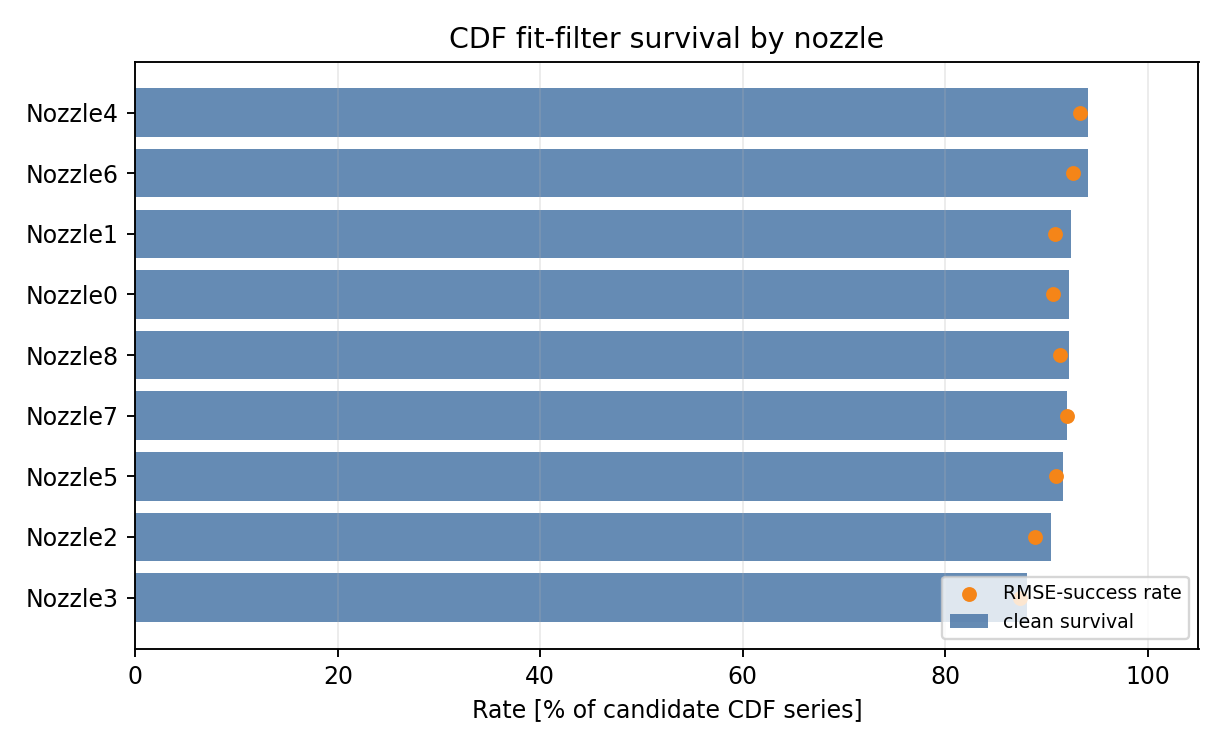
\includegraphics[width=0.88\linewidth]{images/filter_survival_cdf_by_nozzle.png}
\caption{基于恢复后的 PC 归档重新生成的 CDF 穿深 q1 过滤存活率。图中报告全部九个喷嘴族（包括 Nozzle0）的候选总序列数、clean 序列数和通过比例。}
\label{fig:filter-survival-cdf-nozzle}
\end{figure}

\begin{table}[t]
\centering
\footnotesize
\input{../generated/current/data_attrition_tex.tex}
\caption{使用共同 raw 轨迹分母的轨迹流失表。该自动生成表避免把不同总体上的百分比相乘；每道门限都以 raw CDF 穿深 plume 库为分母报告绝对计数。}
\label{tab:data-attrition-generated-zh}
\end{table}

这一折中是有意的，但边界明确。通过排除含混数据，流程为 Stage~2 提供了较少受光学消失、背景反光和液压延迟对齐错误影响的干净教师目标。Stage~3 随后把这一干净先验与原始、未过滤 CDF 穿深数据重新组合：在高信赖度时间箱中信任原始观测，在覆盖率坍塌处退回 Stage~2 教师。最终得到的是早期原始信号保真度与晚期物理一致性之间的受控插值。

但该设计不会消除过滤本身带来的选择偏置。教师的晚期先验仍以照明良好、无遮挡的 plume 为条件；当 Stage~3 退回教师时，输出应被理解为干净 plume 条件下的延拓，而不是对全部喷嘴几何分布的去偏集合估计。

\textbf{q1 降阶代理模型的总体评价。} 综合上述全部证据，\(S(t)=\sigma((t-t_0)/s)\,k_{1/4}\,t^{1/4}\) 应被定位为一个物理上可辩护、数值上稳健的降阶轨迹代理，而非一条新的封闭形式穿深定律。动能指数 \(t^{1/4}\) 继承自 Hiroyasu--Arai \cite{HiroyasuArai1990} 的分阶段穿深观点以及 Zhou 等关于 EOI 后延伸的研究 \cite{ZhouLiLaiWei2019,ZhouLiYi2021}，sigmoid 门则把他们的刚性阶段断点替换为可微过渡，这正是让拟合曲线能作为下游神经网络代理训练目标的结构性前提。
经验上，\(k_{1/4}\) 在 \(\rho_a\) 
%与 \(d_n\) 
上的标度指数与 Hiroyasu--Arai 自由射流预测几乎完全吻合，而更陡的 \(\Delta P\) 指数与存活样本所主导的壁面射流区段相一致；数据本身在 \(99.8\%\) 的拟合中把四参数混合模型坍缩到 \(k_{\mathrm{sqrt}}\!\approx\!0\)，即 \(t^{1/4}\) 是由数据选择而非优化器强加；中段稳健离散度 \(\sim\SI{0.60}{mm}\) 已贴近成像链的光学噪声底线。

模型的两项局限需明确陈述。q1 的三个参数并非独立物理把手——分支幅度与 sigmoid 门之间存在强软冗余，因此 \((k_{1/4}, t_0, s)\) 应被理解为一个耦合的三维平滑曲面，而非三个独立系数；无量纲群 \((\Delta P, \rho_a, d_n)\) 也只能解释 \(\log k_{1/4}\) 变异的 \(R^2\!\approx\!0.33\)。两者都已被代理模型栈的设计所吸收：Stage~1--3 训练神经网络去复现整条评估曲线 \(\hat S(\cdot)\)，而不是去预测参数三元组，因此参数耦合在训练后的输入--输出映射中不会传播；剩余 \(67\%\) 不被维度群解释的轨迹级变异，恰好是 Stage-2 NLL 与 Stage-3 蒸馏所要处理的异方差、工况依赖残余。下游代理的主要工作区间 \(0\)--\(\SI{1.5}{ms}\) 落在 q1 拟合的数据主导区段内；上文所讨论的边界膨胀与参数耦合主要影响 \(>\SI{2}{ms}\) 的远场区段，而该区段在 Stage-3 蒸馏架构中本就由教师模型的保守包络主导。

\subsection{工程化特征设计}

在工程化特征架构确定之前，一个较早的九特征 MLP 曾以直接输入压力和喷嘴直径的方式进行训练，结果暴露出一个结构性问题。当前数据集中，喷嘴直径仅有六个观测层级，且并非在所有压力组合下均有覆盖——全部六个直径层级仅出现于狭窄工况族 $(P_{\mathrm{inj}}=\SI{2000}{bar},\;P_{\mathrm{cb}}=4,\;P_{\mathrm{ch}}\in\{5,10,15\}\,\si{bar})$，喷射压力也只有四个层级。图~\ref{fig:sparse-support-topology} 把这一离散采样格直观展示出来：（腔压、喷射压力、直径）的三维网格大部分单元只包含零个或一个观测，而完整六层直径覆盖仅存在于一条窄压力族上。

\begin{figure}[t]
\centering
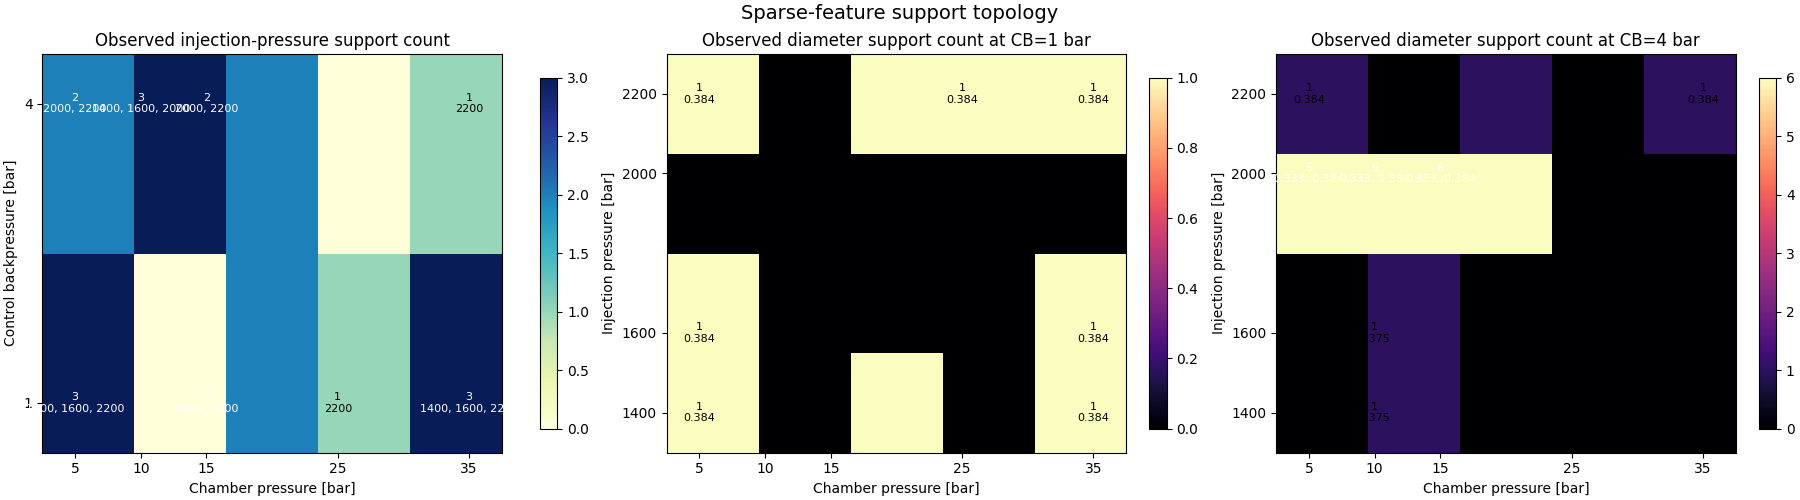
\includegraphics[width=0.96\linewidth]{images/fig_sparse_support_topology.png}
\caption{训练矩阵的稀疏特征支持拓扑。左：在（腔压、控制背压）平面上观测到的喷射压力支持层数，单元内标注了具体可用层级。中、右：在（腔压、喷射压力）平面上，$\mathrm{CB}=\SI{1}{bar}$ 与 $\mathrm{CB}=\SI{4}{bar}$ 时观测到的喷孔直径支持层数。大部分单元只有零个或一个直径层级；完整六层直径覆盖仅出现在狭窄工况族 $(P_{\mathrm{inj}}=\SI{2000}{bar},\;\mathrm{CB}=4,\;P_{\mathrm{ch}}\in\{5,10,15\}\,\si{bar})$ 上。}
\label{fig:sparse-support-topology}
\end{figure}

由于光滑 MLP 把这些输入视为连续变量，它会在直径轴和压力轴上产生数据无法约束的导数结构。图~\ref{fig:sparse-diameter-interpolants} 给出 $t=\SI{0.85}{ms}$ 时对直径轴做密集扫描的结果：在相邻观测层级之间，预测均值曲线每个切片出现五到六次梯度符号变化，自动微分梯度峰值在约 \SI{0.05}{mm} 的支持跨度上达到 $\sim\!\SI{4e4}{}$，即曲率范数达到 $10^7$ 量级；同样的诊断对喷射压力则在稀疏支持切片上产生非单调、不受约束的外推。其根本原因是结构性的——光滑 MLP 被要求从本质上离散的采样格上学习具有物理意义的连续规律，仅靠加大正则化只能以牺牲全局容量为代价抑制不稳定性。修订后的架构因此从源头上解决了这一问题，直接移除了这些稀疏输入。

\begin{figure}[t]
\centering
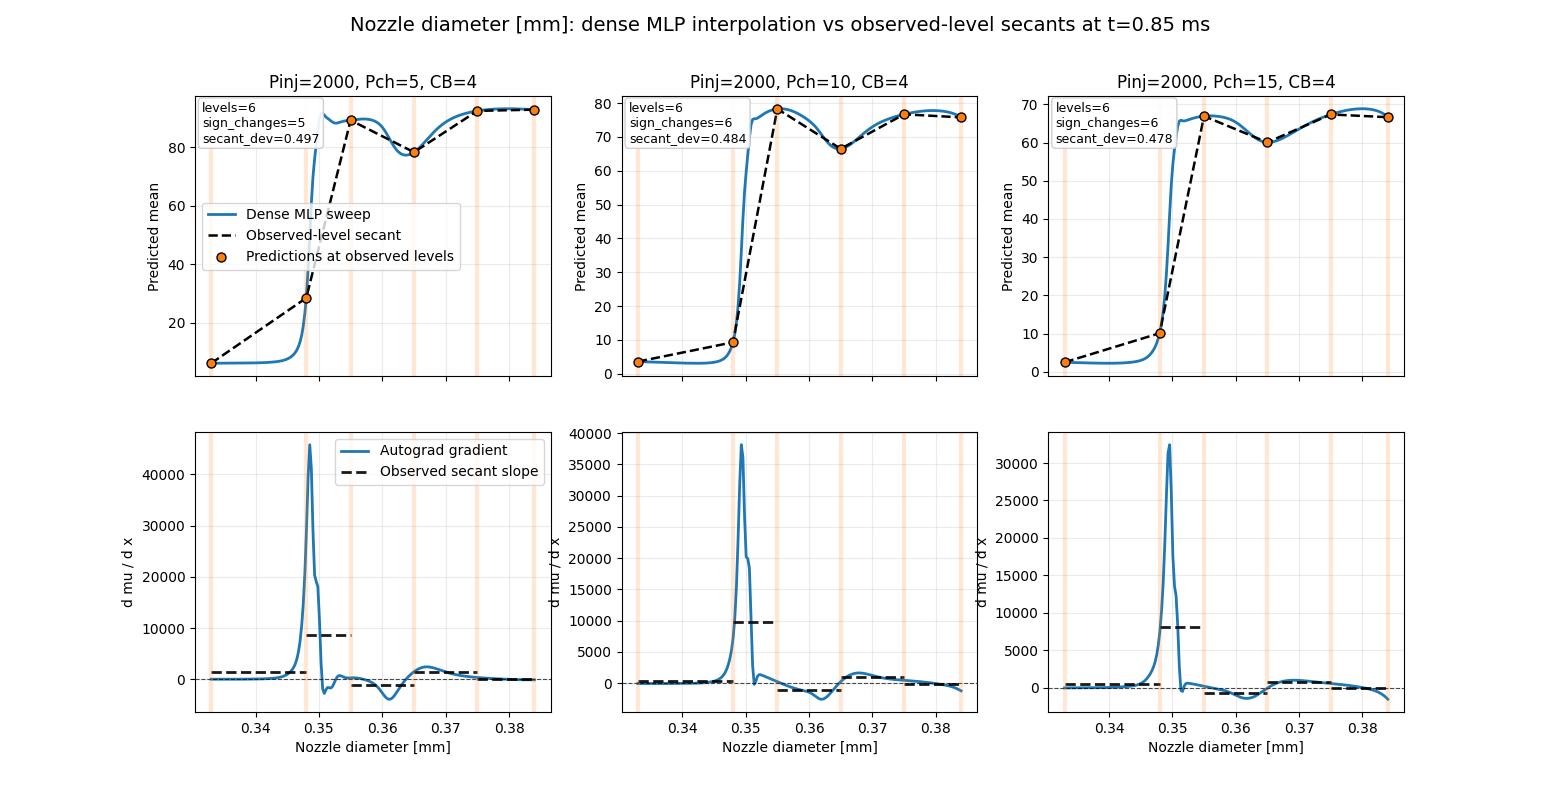
\includegraphics[width=0.98\linewidth]{images/fig_sparse_diameter_interpolants.png}
\caption{直接特征基线下，三个工况点（每列一个）在 $t=\SI{0.85}{ms}$ 时沿喷孔直径轴的 MLP 密集插值。上排：预测均值（蓝色）与穿过六个直径观测层级（橙色）的截线（黑色虚线）对比。下排：自动微分得到的梯度 $\partial\mu/\partial d_n$（蓝色）与观测层级间的截线斜率（黑色虚线）对比。MLP 在每个切片上产生五到六次梯度符号变化，并在 \SI{0.05}{mm} 的支持跨度上出现 $10^4$ 量级的梯度尖峰，这些结构均不受数据约束。}
\label{fig:sparse-diameter-interpolants}
\end{figure}

修订后的代理模型将四个弱支持的压力和直径输入替换为一个硬物理缩放群。Hiroyasu--Arai 破碎后分支 \cite{HiroyasuArai1990} 提供了量纲动机：
\[
S(t)\;\propto\;K_p\!\left(\frac{\Delta P}{\rho_a}\right)^{1/4}d_n^{1/2}\,t^{1/2},
\]
其中 H--A 理论将 $\Delta P^{1/4}$ 分配给压差群。然而，上文所述的经验标度回归在注射中段时间窗口内发现 $\Delta P$ 的经验指数约为 $0.52$，约为 H--A 值的两倍，因此幅度尺度更新为以数据为依据的形式：
\[
A\;=\;\Delta P^{0.5}\cdot\rho_a^{-0.25}\cdot d_n^{0.5},
\]
该量由测试矩阵 JSON 计算得到。该形式保留了经验回归表现良好的 H--A $\rho_a^{-1/4}$ 与 $d_n^{1/2}$ 指数，同时以数据支持的 $\Delta P^{0.5}$ 替代 H--A 的 $\Delta P^{1/4}$。对于 Nozzle1--Nozzle8，气缸密度直接取自记录的腔内气体密度；对于只记录腔内环境压力的 Nozzle0，则按对 Nozzle1--8 数据标定的线性律 $\rho_a=\SI{5}{kg/m^3}\times P_{\mathrm{ch}}/\SI{4.42}{bar}$ 反推 $\rho_a$。

在第一个设计迭代中，将四个稀疏输入完全折叠进 $A$，作为五特征"仅缩放"基线
\[
[\,t_{\mathrm{norm}},\;\theta_{\mathrm{tilt},z},\;n_{\mathrm{plumes},z},\;t_{i,z},\;P_{\mathrm{cb},z}\,],
\]
$A$ 仅作为目标除数，不进入输入。训练目标被重参数化为无量纲穿深 $\hat{S}(t)=S(t)/A$，网络预测 $\hat{\mu}$ 与 $\log\hat{\sigma}^2$，物理量在推理时通过 $\mu_S=A\,\hat{\mu}$、$\sigma_S=A\,\hat{\sigma}$ 精确还原。该基线的 Stage-1 测试 MAE 为 \SI{8.05}{mm}，Stage-2 测试 MAE 为 \SI{9.28}{mm}。

然而，把 $P_{\mathrm{inj}}$ 与 $P_{\mathrm{ch}}$ 完全压缩进 $A$，会丧失两者超出固定 $\Delta P^{0.5}$ 指数所能捕捉范围的独立解释力。标度回归在固定 $\Delta P$ 条件下还估计出非零的腔压系数（中段注射窗口约 $-0.21$ 至 $-0.27$），表明 $P_{\mathrm{inj}}$ 与 $P_{\mathrm{ch}}$ 携带独立的结构信息，无法完全折叠进 $\Delta P$ 一项。此外，全局 $\Delta P^{0.5}$ 指数是一种均场近似；工况空间内的局部非线性残差在 $P_{\mathrm{inj}}$ 与 $P_{\mathrm{ch}}$ 缺席时将无从学习。喷孔直径 $d_n$ 则情况不同：它在数据集中只有六个离散层级，且在条件矩阵中存在严重共线性（见图~\ref{fig:sparse-support-topology}），即便作为独立输入重新引入也无法提供可信的连续信号；因此 $d_n$ 继续保留在 $A$ 内，其效应由 H--A 物理先验来承载。

基于这一分析，最终采用七特征"缩放加残差压力"形式
\[
[\,t_{\mathrm{norm}},\;\theta_{\mathrm{tilt},z},\;n_{\mathrm{plumes},z},\;t_{i,z},\;P_{\mathrm{cb},z},\;\log P_{\mathrm{inj},z},\;\log P_{\mathrm{ch},z}\,],
\]
$A$ 继续作为目标除数处理直径与主要压力的量纲依赖，$\log P_{\mathrm{inj}}$ 与 $\log P_{\mathrm{ch}}$ 作为额外输入，使网络能够学习超出 H--A 固定指数的残余压力结构。与五特征基线相比，Stage-1 测试 MAE 从 \SI{8.05}{mm} 降至 \SI{2.91}{mm}，Stage-2 测试 MAE 从 \SI{9.28}{mm} 降至 \SI{5.63}{mm}，表明残余压力特征携带了在五特征框架下被固定指数所遮蔽的有效信息。

在任何优化之前，物理标度验证流程在实际数据集上检验缩放假设：它将每条轨迹除以自身的 $A$，并计算 $\hat{S}(t)$ 对稀疏特征的线性回归 $R^2$。在七特征生产 run 中，该检验通过——稀疏特征 $R^2$ 从物理目标上的 $0.32$ 降至缩放目标上的 $0.016$——证实 $A$ 已解释了主要的直径与压力依赖性，而 $\log P_{\mathrm{inj}}$ 与 $\log P_{\mathrm{ch}}$ 轴上学习的是 $A$ 所未覆盖的残余结构。若检验失败，训练默认中止，使得物理先验在实际数据集上可证伪而非默认成立。嵌入 $A = \Delta P^{0.5}\cdot\rho_a^{-0.25}\cdot d_n^{0.5}$ 中的经验导出指数携带着一个经验上可验证的预测：训练协议在任何权重更新之前会对这一预测进行确认或拒绝。

Stage~1 与 Stage~2 共用一套组感知数据划分：按整组工况标识符——由喷嘴型号、喷射压力、腔内环境压力与喷射持续时间共同定义——分配训练、验证、测试集，防止共享同一工况点的曲线之间发生泄漏。若不施加这一约束，按轨迹随机划分会使网络在训练集中见过几乎相同工况的曲线后，对测试集的误差仅反映工况内平滑性，而非跨工况域的泛化能力。因此，组感知划分是保证报告的测试集指标可被解释为跨不同工况的插值性能——而非工况内记忆性能——的结构性保障。Stage~2 从 Stage-1 工程化 run 目录热启动并复用其 scaler 状态，保证两个阶段的变体选择与 $A$ 缩放完全一致。

\subsection{无量纲目标上的 Stage-1 MSE 基线}

Stage~1 在代表性轨迹子集上训练确定性均值模型。对于每个文件级工况组，在 $t_{\mathrm{far}}=\SI{5}{ms}$ 处评估 q1 拟合曲线，计算该时刻的组中位穿深，并保留最接近该中位的行作为 Stage-1 代表性轨迹。该过程产出 599 条代表性轨迹，按组划分为 421/89/89 条训练/验证/测试轨迹。

作用于无量纲目标 $\hat{S}$ 的损失为
\[
\begin{aligned}
\mathcal{L}_{\mathrm{stage1}}
=\;&
\operatorname{MSE}\!\left(\hat{\mu},\hat{S}\right)
+\lambda_{\mathrm{var}}
\mathbb{E}\!\left[\left(\log \hat{\sigma}^2-c_0\right)^2\right]\\
&+\lambda_{1}
\mathbb{E}\!\left[\operatorname{ReLU}\!\left(-\frac{\partial \mu_S}{\partial t}\right)^2\right]
+\lambda_{2}
\mathbb{E}\!\left[g(t)\operatorname{ReLU}\!\left(\frac{\partial^2 \mu_S}{\partial t^2}\right)^2\right],
\end{aligned}
\]
其中 $c_0=-2$ 为对数方差先验中心，$g(t)=\sigma((t-t_c)/\tau_c)$ 将凹性惩罚门控至瞬态区域之后，导数惩罚在物理重建 $\mu_S=A\,\hat{\mu}$ 上计算，以确保单调性与凹性约束在可观测尺度上生效。当前 run 采用 \(\lambda_{\mathrm{var}}=10^{-3}\)、\(\lambda_1=5\times10^{-5}\)、\(\lambda_2=5\times10^{-4}\)、\(t_c=\SI{0.9}{ms}\)、\(\tau_c=\SI{0.05}{ms}\)。网络为三隐层 MLP，维度 $[512,512,128]$，平滑门控激活，随机单元屏蔽（率 0.3），使用解耦权重衰减自适应矩优化器配合梯度裁剪及早停。Stage-1 run 在测试集上达到物理 MAE \SI{2.91}{mm}，留出集指标连同其他两阶段一并汇总于表~\ref{tab:model-summary}。

\subsection{Stage-2 异方差 NLL 扩展}

Stage~2 从 Stage-1 checkpoint 热启动，将训练集扩展至所有经过筛选的轨迹，并以缩放目标上的异方差高斯负对数似然替换 MSE 数据拟合项：
\[
\begin{aligned}
\mathcal{L}_{\mathrm{stage2}}
&=
\mathbb{E}\!\left[
\frac{1}{2}
\left(
\log \hat{\sigma}^{2}
+\frac{(\hat{S}-\hat{\mu})^{2}}{\hat{\sigma}^{2}}
\right)\right]
\\
&\quad
+\lambda_{1}\,
\mathbb{E}\!\left[
\operatorname{ReLU}\!\left(-\frac{\partial \mu_S}{\partial t}\right)^{2}
\right]
+\lambda_{2}\,
\mathbb{E}\!\left[
g(t)\operatorname{ReLU}\!\left(\frac{\partial^{2}\mu_S}{\partial t^{2}}\right)^{2}
\right],
\\
\hat{\sigma}^{2}
&=\exp(\log\hat{\sigma}^{2})+\varepsilon.
\end{aligned}
\]
导数惩罚仍然在物理空间重建 $\mu_S=A\,\hat{\mu}$ 上计算，特征映射与 Stage~1 完全相同，确保两个阶段的 $A$ 缩放与变体选择一致。当前 Stage~2 run 采用 \(\lambda_1=5\times10^{-5}\)、\(\lambda_2=5\times10^{-5}\)、\(t_c=\SI{0.5}{ms}\)、\(\tau_c=\SI{0.05}{ms}\)。行表扩展至 71,700 条经过筛选的 q1 轨迹，保留所有通过拟合级掩码以及组内远时刻 z-score 过滤的行。数据划分在 工况分组标识符 层级完成，而不是在单条 plume 轨迹层级完成，因此同一物理工况下的轨迹不会同时泄漏到训练、验证和测试分区中。每条轨迹在 \SIrange{0}{5}{ms} 内采样 512 个时间点，因此生产 Stage-2 训练集共包含 36,710,400 个逐点样本：训练集为 49,908 条轨迹，验证集为 10,961 条轨迹，测试集为 10,831 条轨迹。

保留下来的轨迹覆盖了生产训练集的工况范围：控制背压从 1 到 \SI{4}{bar}，喷射压力从 1,400 到 \SI{2,200}{bar}，喷射持续时间从 340 到 \SI{1,200}{\micro\second}，拟合远时刻穿深从 \SI{26.2}{mm} 到 \SI{217.3}{mm}。因此 Stage~2 学到的并不是单一中位曲线，而是在异常值剔除后仍然存在的组内 plume 差异与重复实验差异。异方差输出用于把纯 MSE 目标会混在一起的两个量分开：条件平均穿深轨迹，以及围绕该平均轨迹的条件离散度。

训练沿用 Stage~1 的特征映射与 scaler 状态。输入向量仍包含归一化时间坐标、$\theta_z$、$N_{\mathrm{plume},z}$、$\Delta t_{\mathrm{inj},z}$、$p_{\mathrm{back},z}$、$\log P_{\mathrm{inj},z}$ 和 $\log P_{\mathrm{ch},z}$（共七个特征），网络仍为三隐层 MLP，维度为 $[512,512,128]$，并从 Stage-1 checkpoint 热启动。Stage~2 run 使用解耦权重衰减自适应矩优化器，学习率 \(8\times10^{-4}\)，解耦权重衰减系数 \(10^{-4}\)，batch size 为 96，梯度裁剪范数为 1.0，对数方差边界为 \([-10,6]\)，早停耐心为 35。因此，该阶段在数据拟合项上的有意变化，是把确定性 MSE 替换为带学习方差输出的高斯 NLL。

\begin{table}[t]
\centering
\footnotesize
\setlength{\tabcolsep}{3pt}
\begin{tabular}{|L{0.20\linewidth}|L{0.08\linewidth}|L{0.14\linewidth}|L{0.13\linewidth}|L{0.12\linewidth}|L{0.12\linewidth}|}
\hline
划分 & Epoch & 逐点样本数 & Loss / 缩放 NLL & 物理 MAE & 平均预测标准差 \\
\hline
最佳验证 epoch 的训练集 & 116 & 25{,}552{,}896 & -0.188 / -0.190 & \SI{5.95}{mm} & \SI{7.67}{mm} \\
验证集，最佳 checkpoint & 116 & 5{,}612{,}032 & -0.323 / -0.323 & \SI{5.11}{mm} & \SI{7.08}{mm} \\
验证集，早停 epoch & 151 & 5{,}612{,}032 & -0.317 / -0.317 & \SI{5.12}{mm} & \SI{7.05}{mm} \\
测试集，恢复最佳 checkpoint & 151 & 5{,}545{,}472 & -0.240 / -0.240 & \SI{5.63}{mm} & \SI{7.61}{mm} \\
\hline
\end{tabular}
\caption{Stage-2 epoch 级损失摘要。最佳验证 NLL 出现在第 116 个 epoch；训练在第 151 个 epoch 早停。测试行是在早停后写入的，但测试评估前模型权重已恢复至最佳验证 checkpoint。}
\label{tab:stage2-epoch-loss}
\end{table}

表~\ref{tab:stage2-epoch-loss}显示，留存测试集 MAE 为 \SI{5.63}{mm}，与验证集 MAE 接近。Stage-2 测试集 MAE 在数值上高于 Stage-1 的 \SI{2.91}{mm}，但两者并不直接可比：Stage-1 在 599 条代表性轨迹上训练（每个工况组取一条），Stage-2 则在 49{,}908 条涵盖组内 plume 间变异和完整工况范围的轨迹上训练；更宽、更异质的训练集是设计的意图，而非精度标准的放宽。平均预测标准差为 \SI{7.61}{mm}，仍大于逐点误差尺度。这正是该阶段所需要的行为：模型不再被迫把所有 plume 间残差变化都压入均值函数，而是给出非零的条件不确定性，供后续概率性风险筛查与蒸馏阶段使用。该 checkpoint 作为后续蒸馏阶段的教师模型。

\begin{figure}[t]
\centering
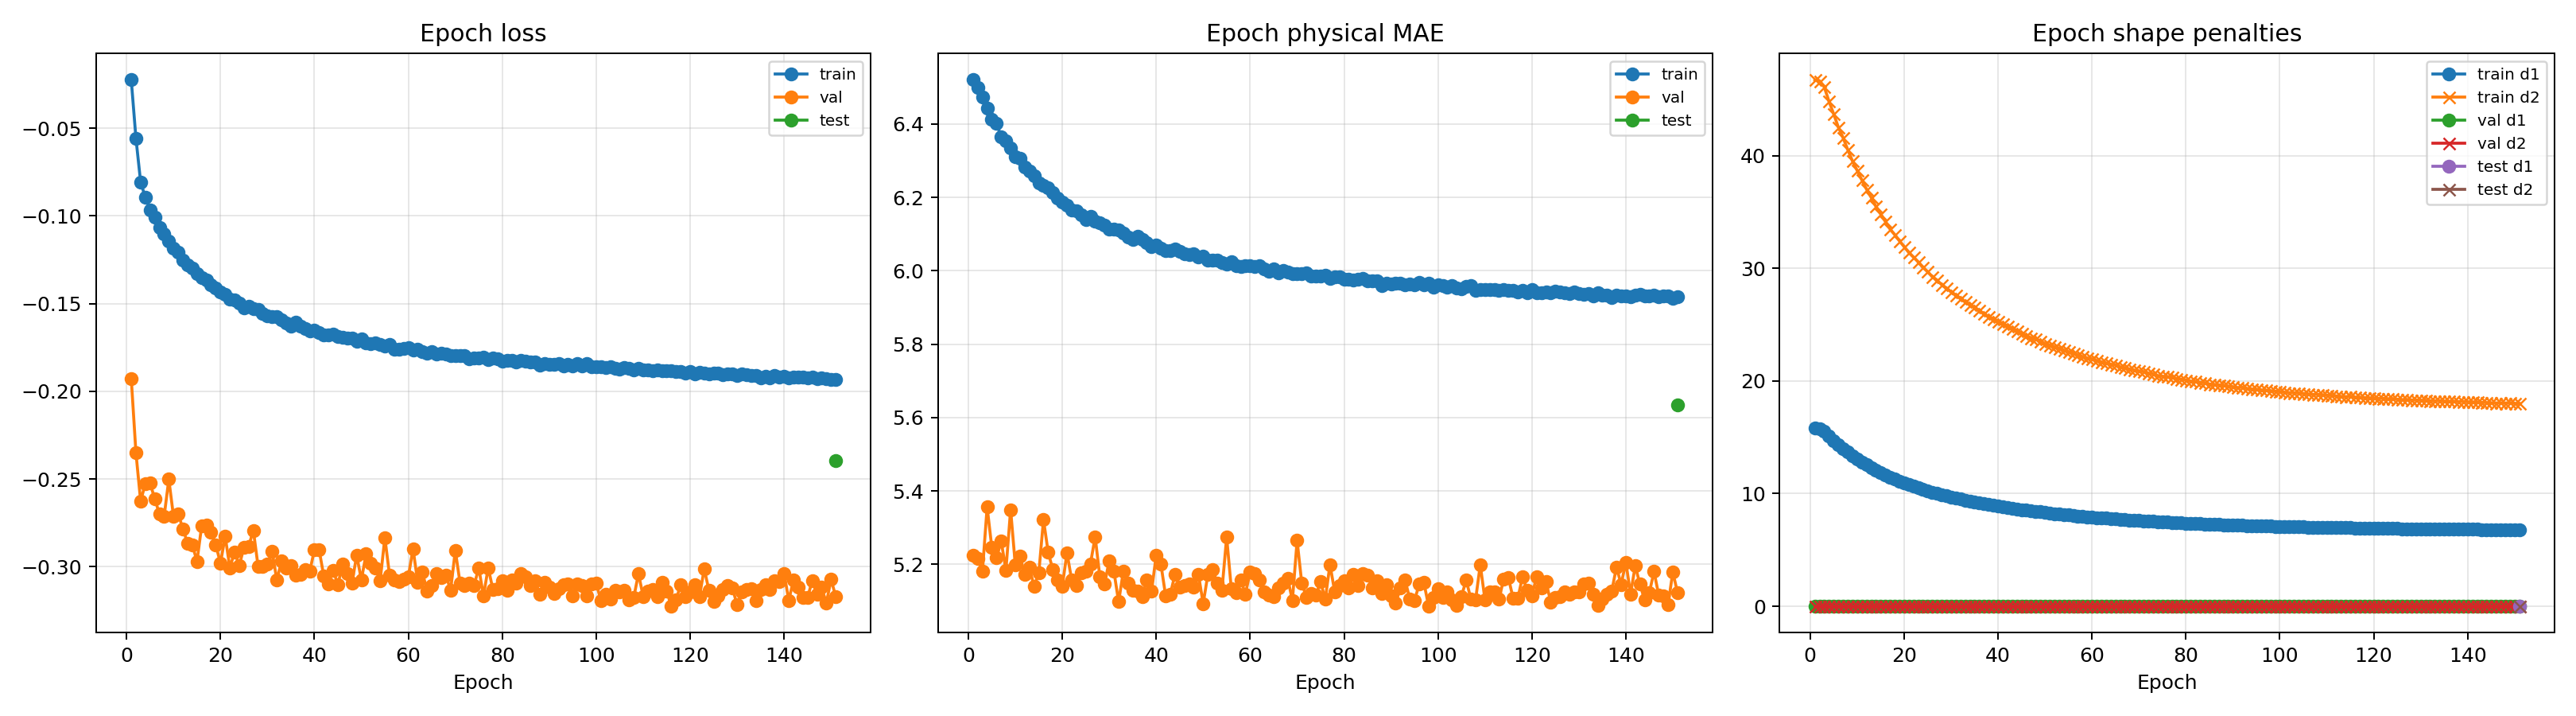
\includegraphics[width=0.85\linewidth]{images/stage2_loss_curves.png}
\caption{Stage-2 NLL 训练曲线，展示逐 epoch 的训练集与验证集高斯 NLL。最佳验证 checkpoint 出现在第 116 个 epoch；早停在第 151 个 epoch 终止训练。}
\label{fig:stage2-loss-curves}
\end{figure}

\subsection{原始 CDF 穿深蒸馏与喷射起始精化}

NLL 阶段在拟合训练目标上产出了良好的异方差预测，但拟合曲线在整个时间轴上的忠实程度并不均匀。在注入起始附近，绝对穿深很小，任何时间偏移、拟合延迟模糊或平滑性先验都会产生相对较大的分数误差，因此每条预测曲线的最早部分仍然由拟合目标先验主导，而不是由直接观测到的原始羽流动力学决定。图~\ref{fig:stage2-toy-inference-early-time}以代表性玩具推理扫描展示了这一现象。

\begin{figure}[t]
\centering
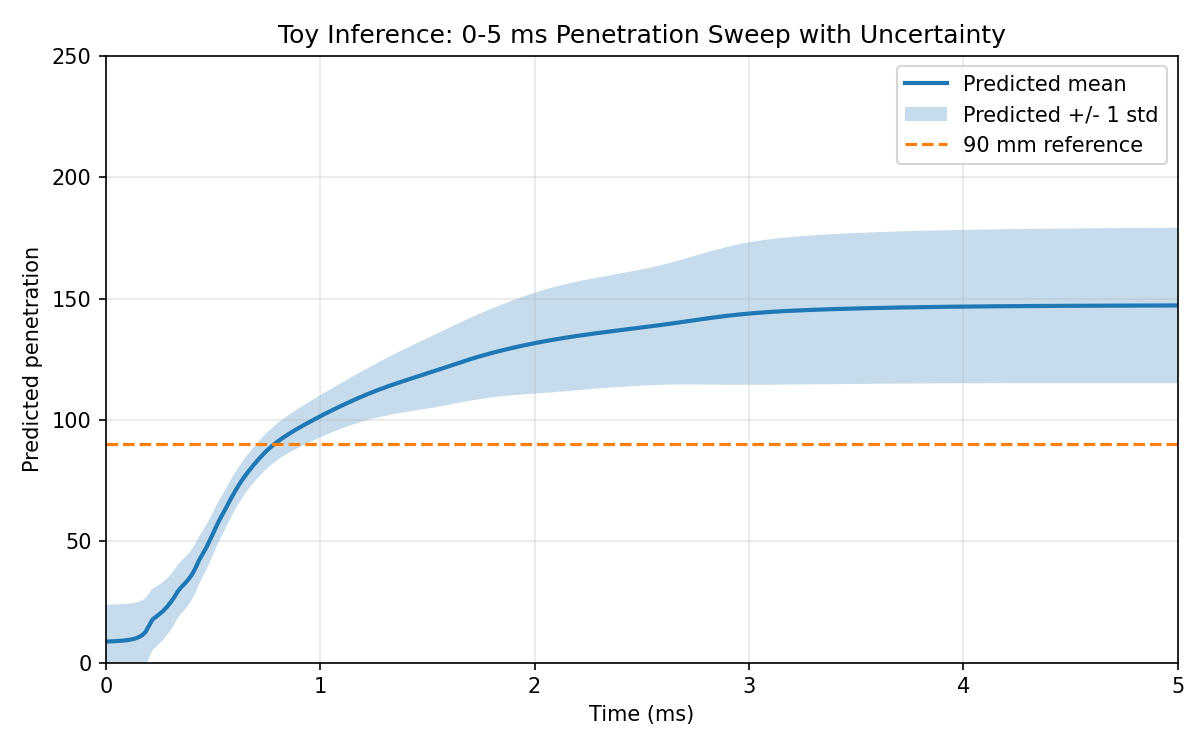
\includegraphics[width=0.82\linewidth]{images/stage2_toy_inference_2000bar_5bar.png}
\caption{Stage-2 NLL 模型在代表性 \(\SI{2000}{bar}\)、\(\SI{5}{bar}\) 工况下的玩具推理结果。预测整体平滑且具有不确定性感知，但轨迹最早部分仍然主要由拟合目标先验塑造，这正是后续蒸馏精化的动机。}
\label{fig:stage2-toy-inference-early-time}
\end{figure}

为了在原始 CDF 穿深观测上精化早期时间动态，同时防止在晚期稀疏区域崩塌，一个知识蒸馏阶段被实现并归档为独立的学生 checkpoint。Stage-2 NLL 模型作为固定教师；学生网络继承教师权重，并通过原始 CDF 穿深与教师指导的联合训练进一步精化。

\textbf{CDF 穿深覆盖率区制。}  由于原始 CDF 穿深序列存在右删失问题（到 $t\approx\SI{3}{ms}$ 时，许多工况已损失超过 70\% 的测量值），无法在时间轴上均匀地施加直接的原始监督。对于每个工况组，原始观测被分入 $[0,5]\,\si{ms}$ 上 $\Delta t=\SI{0.1}{ms}$ 的时间箱，每箱的平滑样本数作为覆盖率代理，确定三个互斥区制：高信赖度原始区间（平滑覆盖率 $\geq$ 峰值的 70\%）、不确定原始区间（覆盖率在 20\%--70\% 之间）、纯教师外推区间（覆盖率低于 20\% 或每箱少于 4 个样本）。区制转换需要至少两个连续时间箱，以防止孤立下跌触发过早的区制切换。

这里的 70\%/20\% 覆盖率边界是保守的工程区制规则，而不是完整网格搜索的最优解。当前已完成的 Stage~3 消融主要支持两个结论：关闭早期 anchor 能降低全局低估偏差，且在可靠原始区间保留轻度 KD 混合优于完全移除教师约束；覆盖率边界与 \(\sigma_{\mathrm{ref}}\) 的系统性敏感性超出当前消融范围，构成相应局限。

\begin{figure}[t]
\centering
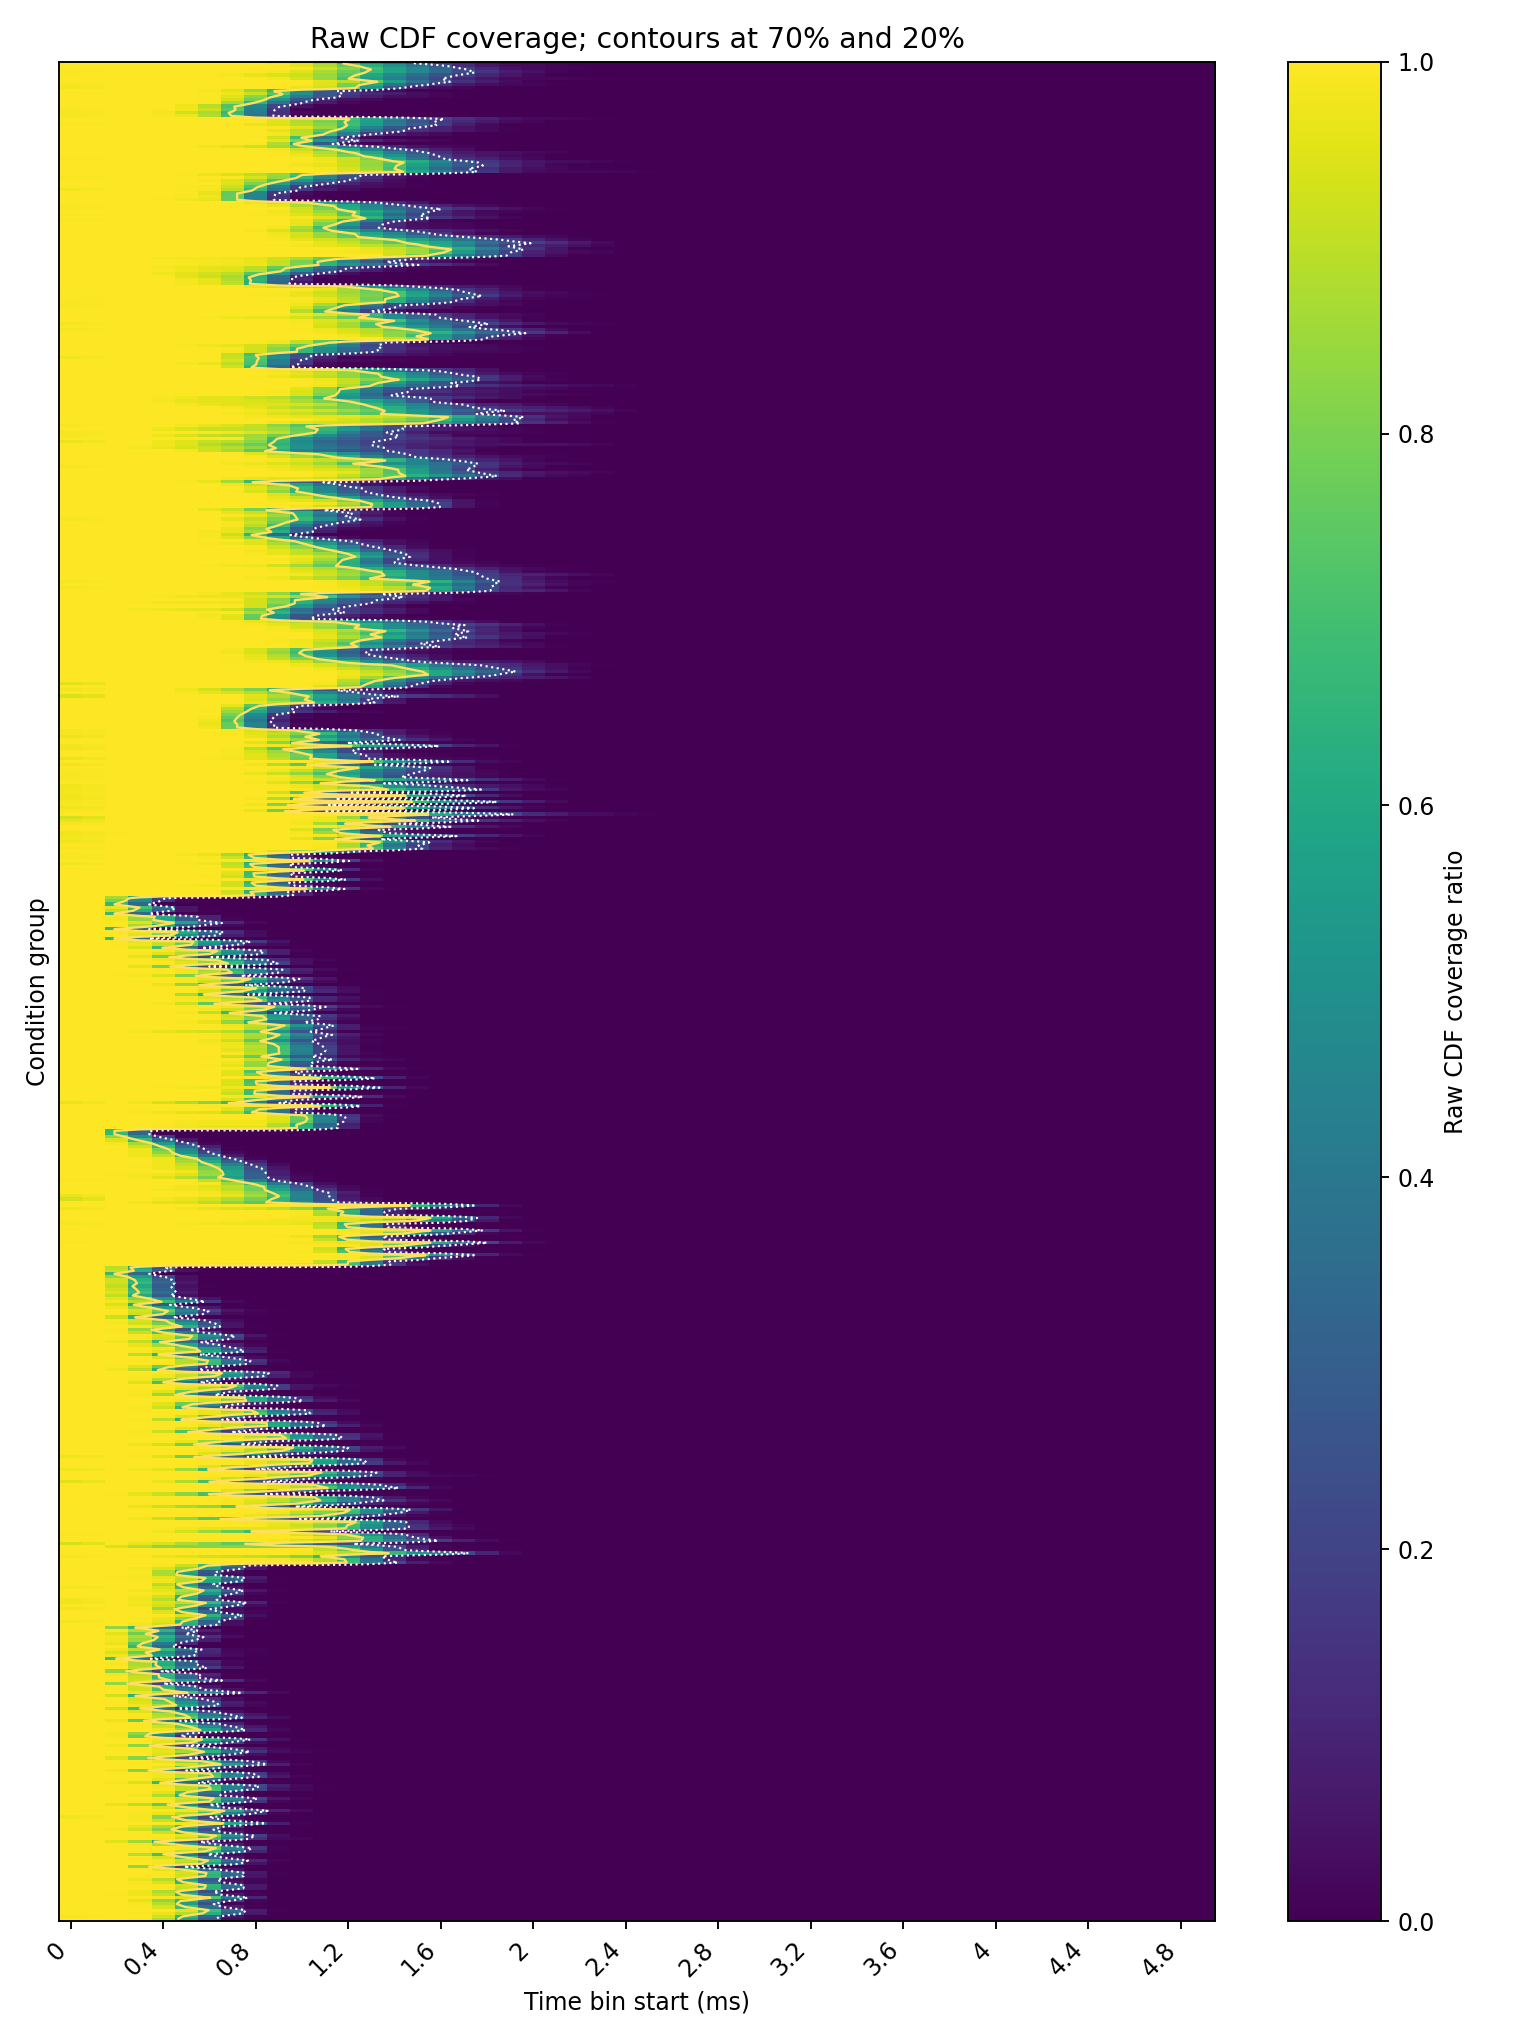
\includegraphics[width=0.94\linewidth]{../generated/current/raw_coverage_heatmap.png}
\caption{用于审计 70\%/20\% 分区边界的自动生成 raw-CDF 覆盖率热图。等值线标记 reliable-to-uncertain 与 uncertain-to-teacher-only 两个阈值。}
\label{fig:raw-coverage-heatmap-generated-zh}
\end{figure}

图~\ref{fig:raw-uncertain-teacher-gaussian} 展示了为什么这里需要蒸馏，而不是简单采用单一监督来源。在代表性的 \(\SI{2000}{bar}\)、\(\SI{5}{bar}\) 工况中，剩余的不确定原始区间 CDF 穿深点仍然携带局部观测信息，但它们已经是教师预测分布中逐渐变稀、带有选择偏置的子集。因此，教师 Gaussian 在这里提供了对原始趋势的稳定延续。

\begin{figure}[p]
\centering
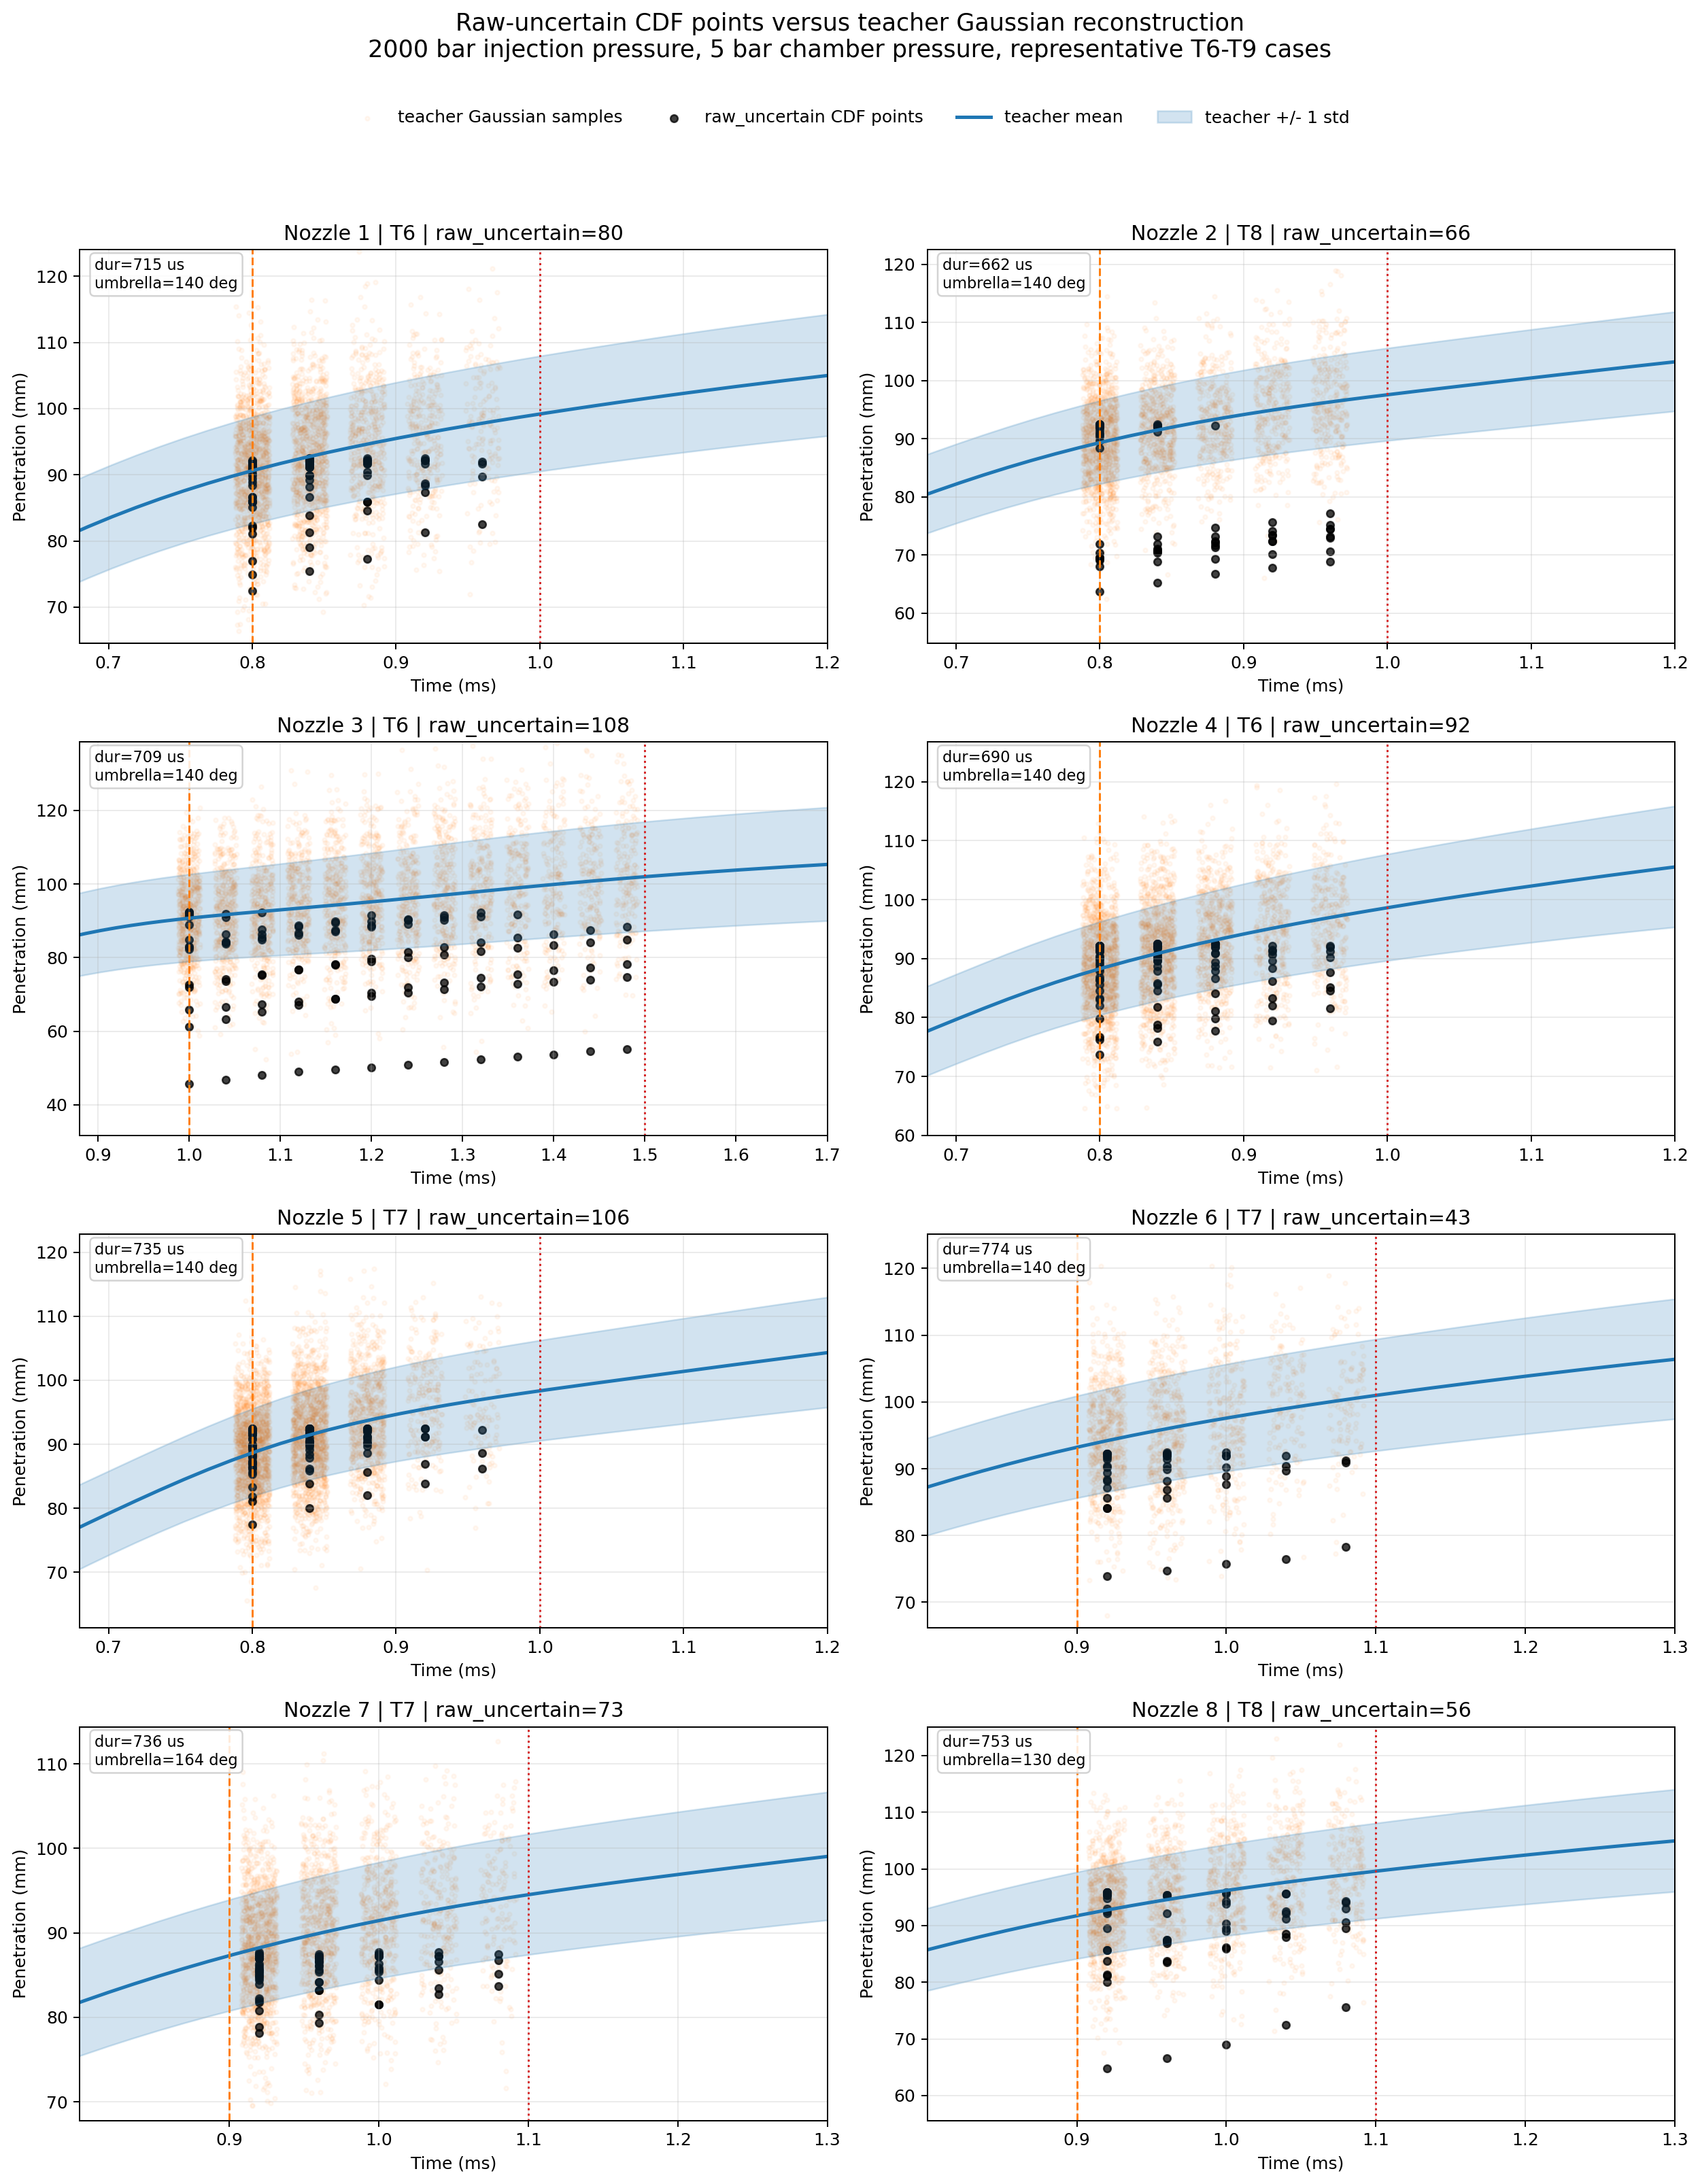
\includegraphics[height=0.88\textheight,keepaspectratio]{images/raw_uncertain_vs_teacher_gaussian_2000bar_5bar.png}
\caption{代表性 不确定原始区间 CDF 穿深点与 Stage~2 教师 Gaussian 重建的对比，工况为 \(\SI{2000}{bar}\) 喷射压力和 \(\SI{5}{bar}\) 腔压。黑点为不确定区制中仍保留下来的原始 CDF 穿深观测，橙色点为在相同时间处从教师 Gaussian 抽样得到的样本，蓝色曲线与阴影分别为教师均值和 \(\pm1\sigma\)。该图说明，一旦覆盖率开始崩塌，Stage~3 目标需要把原始监督与教师引导结合起来。}
\label{fig:raw-uncertain-teacher-gaussian}
\end{figure}

\textbf{监督权重。}  每个网格点接收两个独立的权重通道：

\begin{center}
\begin{tabular}{lcc}
\toprule
区制 & 原始权重 $w_{\mathrm{raw}}$ & 知识蒸馏权重 $w_{\mathrm{kd}}$ \\
\midrule
高信赖度原始区间  & 1.0 & 0.25 \\
不确定原始区间 & 0.0 & 1.0  \\
纯教师外推区间  & 0.0 & 0.75 \\
\bottomrule
\end{tabular}
\end{center}

两个通道还通过全局时间箱再平衡权重（逆频率，裁剪至 $[0.5,2.0]$）进一步调制。在 高信赖度原始区间 箱中，原始 NLL 为主要信号，辅以轻度 KD 正则化；在 不确定原始区间 箱中，原始监督被丢弃，教师 KL 散度占主导；在 纯教师外推区间 箱中，KD 权重略有降低，以反映教师在外推区域的不确定性。

\textbf{复合损失函数。}  训练目标为
\[
\mathcal{L} = \mathcal{L}_{\mathrm{raw}} + \mathcal{L}_{\mathrm{KD}} + \lambda_{\mathrm{onset}}\,\mathcal{L}_{\mathrm{onset}} + \lambda_{\mathrm{anchor}}\,\mathcal{L}_{\mathrm{anchor}} + \lambda_{d_1}\,P_{d_1} + \lambda_{d_2}\,P_{d_2},
\]
其中 $\mathcal{L}_{\mathrm{raw}}$ 为物理空间 $(\mu,\sigma^2)$ 相对于原始 CDF 穿深目标的高斯 NLL，由 $w_{\mathrm{raw}}$ 加权；$\mathcal{L}_{\mathrm{KD}}$ 为前向 KL 散度 $D_{\mathrm{KL}}(p_{\mathrm{teacher}}\|p_{\mathrm{student}})$（物理空间，教师到学生方向），由 $w_{\mathrm{kd}}$ 及教师置信因子
\[
w_{\mathrm{conf}}(t) = \mathrm{clamp}\!\left(\frac{\sigma_{\mathrm{ref}}}{\sigma_{\mathrm{teacher}}(t)},\;0.25,\;1.0\right),\quad\sigma_{\mathrm{ref}}=\SI{10}{mm}
\]
共同加权。该因子根据教师不确定度超出参考尺度的程度按比例缩减有效 KD 权重：当 $\sigma_{\mathrm{teacher}}\leq\sigma_{\mathrm{ref}}$ 时教师置信度高，$w_{\mathrm{conf}}=1$；当 $\sigma_{\mathrm{teacher}}\gg\sigma_{\mathrm{ref}}$ 时，$\sigma_{\mathrm{teacher}}(t)$ 反映的是同一工况下 q1 拟合曲线在该时刻外推段内的穿深离散度，而非经验证的物理外推不确定性；此时有效 KD 权重被下调至下界 $0.25$，防止学生在删失的晚期尾部被这一随时间累积的组内离散度所主导。$\mathcal{L}_{\mathrm{onset}}$ 为新增起始 logit 输出相对于斜坡目标 $\min(t/t_{\mathrm{ramp}},1)$ 的二元交叉熵损失，仅在 $t\leq\SI{0.2}{ms}$ 时激活（$\lambda_{\mathrm{onset}}=0.1$）；$\mathcal{L}_{\mathrm{anchor}}$ 为将 $\mu(t\approx0)$ 拉向零的二次惩罚，在前 \SI{0.15}{ms} 内逐渐消退。该项保留在通用目标函数和 baseline run 中（$\lambda_{\mathrm{anchor}}=0.01$），但最终选定的 checkpoint 在消融后采用 $\lambda_{\mathrm{anchor}}=0$，因为早期锚点会引入轻微的系统性低估。$P_{d_1}=\operatorname{ReLU}(-\Delta\mu)^2$ 强制单调性；$P_{d_2}=\operatorname{ReLU}(+\Delta^2\mu)^2$ 在 $t\geq\SI{0.5}{ms}$ 后强制凹性。

\begin{table}[t]
\centering
\footnotesize
\setlength{\tabcolsep}{3pt}
\renewcommand{\arraystretch}{1.18}
\begin{tabular}{@{}L{0.12\linewidth}L{0.24\linewidth}L{0.24\linewidth}L{0.30\linewidth}@{}}
\toprule
阶段 & 数据项与方差/起始项 & 形状先验 & 门控与蒸馏参数 \\
\midrule
Stage~1 &
\(\lambda_{\mathrm{var}}=10^{-3}\), \(c_0=-2\) &
\(\lambda_1=5\times10^{-5}\), \(\lambda_2=5\times10^{-4}\) &
\(t_c=\SI{0.9}{ms}\), \(\tau_c=\SI{0.05}{ms}\) \\
Stage~2 &
异方差 NLL，\(\log\hat{\sigma}^2\in[-10,6]\) &
\(\lambda_1=5\times10^{-5}\), \(\lambda_2=5\times10^{-5}\) &
\(t_c=\SI{0.5}{ms}\), \(\tau_c=\SI{0.05}{ms}\) \\
Stage~3 &
\(\lambda_{\mathrm{onset}}=0.1\), final \(\lambda_{\mathrm{anchor}}=0\) &
\(\lambda_{d_1}=5\times10^{-5}\), \(\lambda_{d_2}=5\times10^{-4}\) &
\(t_c=\SI{0.5}{ms}\), \(\tau_c=\SI{0.05}{ms}\), \(\sigma_{\mathrm{ref}}=\SI{10}{mm}\); \(w_{\mathrm{raw}}=(1.0,0,0)\), \(w_{\mathrm{kd}}=(0.25,1.0,0.75)\) \\
\bottomrule
\end{tabular}
\caption{三阶段训练中影响复现的主要超参数。Stage~1/2 数值来自对应的训练配置快照；Stage~3 数值来自最终 anchor-off run。\(w_{\mathrm{raw}}\) 与 \(w_{\mathrm{kd}}\) 的三元组顺序为高信赖度原始区间、不确定原始区间、纯教师外推区间。}
\label{tab:training-hyperparameters}
\end{table}

\textbf{学生模型架构。}  学生为三输出 MLP，在教师的两个输出 $[\hat\mu,\;\log\hat\sigma^2]$ 基础上增加一个起始 logit。所有共享层从教师 checkpoint 复制；起始头的最终线性层初始化为零（sigmoid $\to0.5$）。所有损失均在物理空间计算，学生和教师输出在评估 $\mathcal{L}_{\mathrm{KD}}$、$\mathcal{L}_{\mathrm{raw}}$ 及形状先验之前乘以每样本的 $A$。

\textbf{训练与结果。}  学生以解耦权重衰减自适应矩优化器（$\mathrm{lr}=3\times10^{-3}$）优化，梯度裁剪范数为~1.0，早停耐心为~20。最终选定的 anchor-off 配置取得最佳验证复合损失~2.230（验证原始 NLL~2.185，验证 KD KL~0.0136，验证起始 BCE~0.320）。在留存测试集上，复合损失为~2.219，其中原始 NLL~2.173、KD KL~0.0136、起始 BCE~0.320，导数惩罚较小（$P_{d_1}\approx8.9\times10^{-5}$，$P_{d_2}\approx2.5\times10^{-4}$）。图~\ref{fig:distillation-loss} 展示了训练曲线；该 checkpoint 在下游筛查任务上的表现汇总于表~\ref{tab:model-summary}。

这些 Stage~3 损失值不能直接与 Stage~2 的 scaled NLL 做优劣比较。Stage~2 在过滤后的轨迹表上优化 q1 拟合目标，而 Stage~3 在另一组 raw/KD 区制总体上混合了 raw CDF 穿深似然、教师--学生 KL、起始监督与形状惩罚。因此，复现管线在导出各阶段指标时显式记录目标总体标签，而不是把所有类似 NLL 的数值放进同一个排行榜。

\begin{figure}[t]
\centering
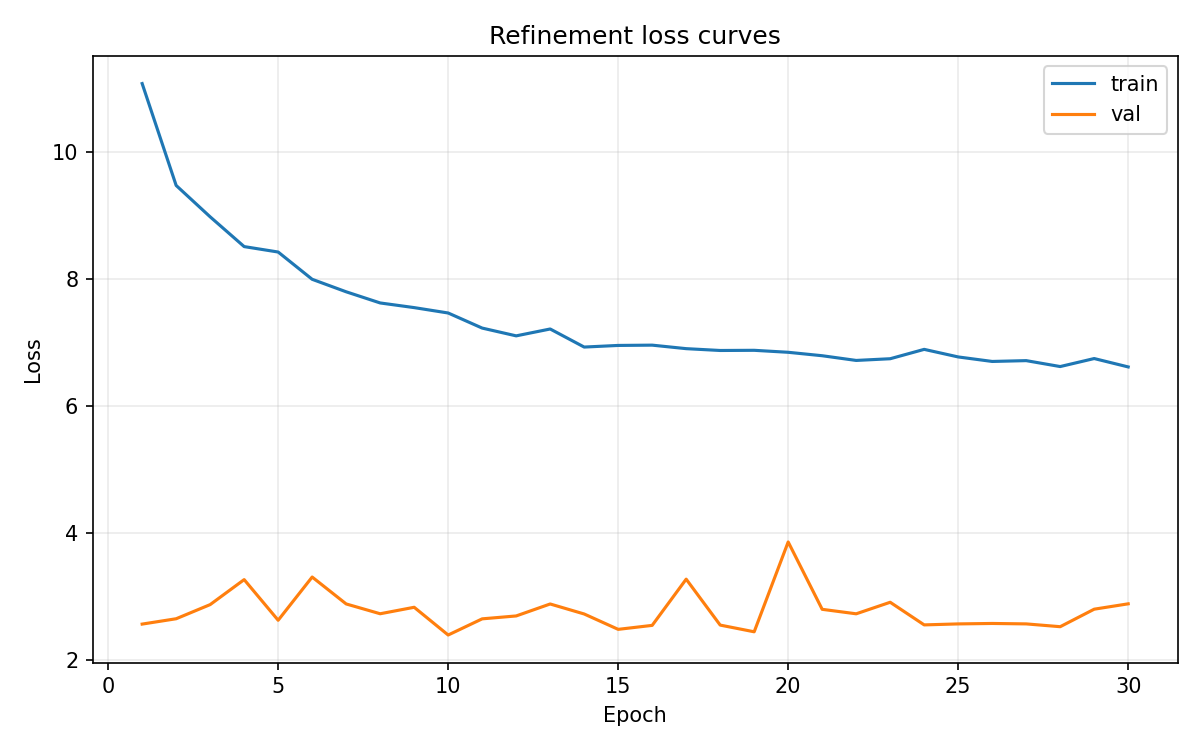
\includegraphics[width=0.92\linewidth]{images/distillation_loss_curves.png}
\caption{最终 anchor-off Stage~3 run 的蒸馏阶段训练曲线。复合损失达到最佳验证值~2.230。}
\label{fig:distillation-loss}
\end{figure}

以上三阶段 surrogate 将在第~5~章中与物理及非参数基线对比评估。以下两个小节描述这些基线的构造协议及所有模型共用的评估规程。

\subsection{物理与非参数基线的构造和拟合协议}\label{sec:baseline-fitting-protocol-zh}

结果章中的 Hiroyasu--Arai、Naber--Siebers 和 Gaussian process 基线均从同一套外部清洗评估表构造，而不是从原始图像像素直接拟合。
因此，基线比较检验的是不同穿深函数族在相同观测定义和相同数据划分下的表现，而不是不同图像处理方法的混合效应。
图像侧输入先经过第~3 章所述的统一流程：对每个视频做喷嘴中心标定、极坐标 plume 条带提取、背景与梯度增强、逐 plume 轴向强度投影、CDF 前沿量化、异常跳变截断、短有效段剔除、像素到毫米转换，以及基于 SOI / 液压延迟的时间对齐。
最终传给基线模型的是逐时间点穿深 \(S(t)\)、同一行的标准化工况特征，以及由测试矩阵 JSON 派生的 \(d_n\)、\(\Delta P\)、\(\rho_a\)、\(A\) 等规范化物理量。

Hiroyasu--Arai 基线使用文献综述中给出的两阶段函数 \(S_{\mathrm{HA}}(t)\)。
报告表中的"校准式"并非直接套用文献常数，而是在训练划分上用 Huber 鲁棒最小二乘拟合 \((k_v,k_p,k_b)\) 的对数参数，随后在验证和测试划分上固定这些参数评估。
对数参数化保证增益和破碎时间比例为正，Huber 损失降低少量图像误检点对全局经验式的杠杆影响。
Naber--Siebers 基线使用延迟平方根形式 \(S_{\mathrm{NS}}(t)=k_{\mathrm{NS}}A\sqrt{\max(t-\tau,0)}\)，其中 \(A=(\Delta P/\rho_a)^{1/4}d_n^{1/2}\)。
报告行拟合 \(\log k_{\mathrm{NS}}\) 和 \(\tau\)，延迟被限制在 \([-0.1,0.8]\,\si{ms}\) 内；角度修正项只作为可选实现存在，最终对比不使用训练集锥角或 oracle 锥角。

为了让物理基线也能进入概率性评价，Hiroyasu--Arai 与 Naber--Siebers 的不确定度不是任意常数。
拟合完成后，训练/验证残差按时间以 \(\SI{0.1}{ms}\) 分箱估计稳健离散度，使用 \(1.4826\,\mathrm{MAD}\) 近似标准差，并施加 \(\SI{0.5}{mm}\) 的方差下限以避免早期低样本分箱产生过窄误差带。
这样得到的 \(\sigma(t)\) 使经验式可报告 1\(\sigma\)、2\(\sigma\) 覆盖率和 CRPS，同时仍保持其均值函数为传统穿深关联式。

Gaussian process 基线则在同一 scaled target 上训练。
它使用 ``a-only'' 五特征集（不含 $\log P_{\mathrm{inj}}$ 和 $\log P_{\mathrm{ch}}$ 的五个基础特征），而非 MLP 生产模型所用的七特征集，
\[
[\,t_{\mathrm{norm}},\;\theta_{\mathrm{tilt},z},\;n_{\mathrm{plumes},z},\;t_{i,z},\;P_{\mathrm{cb},z}\,],
\]
目标为 \(\hat S=S/A\)，预测后再用 \(A\hat\mu\) 和 \(A\hat\sigma\) 返回毫米单位。
实现上采用稀疏异方差 GP：一个稀疏变分 GP 学习均值，另一个 GP 学习对数残差方差；核函数使用带自动相关维度长度尺度的 Mat\'ern \(5/2\) 核，诱导点近似使其能够在外部清洗协议的大样本表上训练。
因此，GP 与 MLP 在目标缩放（均为 $\hat{S}=S/A$）上一致，但 GP 输入为五个特征，少于 MLP 生产模型所用的七个；两者的主要区别在于 GP 用核函数和诱导点近似表达条件函数，而 MLP 用三阶段神经网络和蒸馏损失完成同一任务。

\begin{table}[t]
\centering
\footnotesize
\setlength{\tabcolsep}{3pt}
\begin{tabular}{@{}L{0.18\linewidth}L{0.25\linewidth}L{0.25\linewidth}L{0.24\linewidth}@{}}
\toprule
基线 & 拟合目标与输入 & 可训练参数 & 概率输出方式 \\
\midrule
Hiroyasu--Arai 校准式 &
图像 CDF 穿深 \(S(t)\)；\(t,d_n,\Delta P,\rho_a\) &
\(\log k_v,\log k_p,\log k_b\)，Huber 鲁棒最小二乘 &
时间分箱残差 MAD；\(\sigma_{\min}=\SI{0.5}{mm}\) \\
\midrule
Naber--Siebers 延迟式 &
\(S(t)\)；\(t,A=(\Delta P/\rho_a)^{1/4}d_n^{1/2}\) &
\(\log k_{\mathrm{NS}}\) 与 \(\tau\in[-0.1,0.8]\,\si{ms}\) &
同一残差分箱协议；不使用 oracle 锥角 \\
\midrule
稀疏异方差 GP &
\(\hat S=S/A\)；a-only 标准化特征 &
均值 GP 与对数方差 GP 的核超参数、诱导点和变分参数 &
GP 均值与输入相关方差，经 \(A\) 反缩放为 mm \\
\bottomrule
\end{tabular}
\caption{外部清洗评估中传统物理基线与非参数统计基线的统一构造协议。所有模型使用同一图像处理导出的穿深表、同一组感知划分和同一评估目标。}
\label{tab:baseline-fitting-protocol-zh}
\end{table}

\subsection{评估协议与指标}
\label{sec:evaluation-protocol-zh}

所有模型均在同一来源于外部清洗评估表的留出测试集上进行比较。外部清洗流程在冻结图像归档上重新运行完整的图像处理与目标构造链，生成穿深表，再按组感知方式划分为训练、验证和测试三个子集。测试子集从不用于模型选择或超参数调优；所报告的测试集数值因此是模型未曾影响过的数据上的单次评估结果。

\textbf{点误差指标。} 均方根误差（RMSE）和平均绝对误差（MAE）衡量预测条件均值 $\mu(t)$ 与留出逐点穿深观测之间的准确性。两者均在测试轨迹所覆盖的完整时间范围内计算。由于同一条轨迹内各时间点的误差在时间上相关，有效样本数远小于逐点样本数；所报告数值描述的是跨工况和时刻的平均逐点误差，而非统计独立样本的误差。

\textbf{经验覆盖率。} 异方差模型同时输出条件均值 $\mu(t)$ 和条件标准差 $\sigma(t)$。校准的核心问题是预测不确定度区间在经验上是否可信：在 Gaussian 预测分布下，$68.3\%$ 的观测应落入 $[\mu-\sigma,\,\mu+\sigma]$ 区间，$95.4\%$ 的观测应落入 $[\mu-2\sigma,\,\mu+2\sigma]$ 区间。留出测试集上的经验 $1\sigma$ 覆盖率是每个概率模型的主要校准指标：高于 $68.3\%$ 说明区间保守（方差过大），低于该值说明预测过于自信（方差过小）。对于物理基线，$\sigma(t)$ 为基于训练残差估计的时间分箱稳健扩展；对于 MLP 各阶段，$\sigma(t)$ 直接来自网络输出。

\textbf{连续排名概率评分（CRPS）。} CRPS 通过以下公式评估预测累积分布函数 $F$ 与标量观测 $y$ 之间的差异：
\[
\mathrm{CRPS}(F,y) = \int_{-\infty}^{\infty}\!\left(F(z)-\mathbf{1}[z\geq y]\right)^2\mathrm{d}z.
\]
在均值为 $\mu$、标准差为 $\sigma$ 的 Gaussian 预测分布下，上式可化简为闭合表达式，同时奖励准确性（$|\mu-y|$ 小）和校准性（$\sigma$ 既不过宽也不过窄）。CRPS 越低越好；一个完全准确且完全尖锐的点预测对应 $\mathrm{CRPS}=0$。

\textbf{留一喷嘴族评估。} 标准组感知划分在训练和验证子集中保留所有喷嘴族，检验的是支持工况域内跨压力和喷射时长组合的插值能力。为了在物理上有意义的方向上探测分布外鲁棒性，还额外进行了留一喷嘴族评估：将某一喷嘴族的所有工况从训练和验证子集中移除，在剩余喷嘴族上重新训练模型，并仅在留出喷嘴族上评估性能；对每个喷嘴族依次重复上述过程。由于各喷嘴族在喷孔直径、plume 数量和早期瞬态喷雾形成动力学上均存在差异，留一族评估检验的是：当某种喷嘴几何形状在训练中从未出现时，分阶段结构是否仍能泛化——这是当前数据集所能提供的最严苛的外推场景。两种评估协议的结果均在第~5~章中报告。

\subsection{原型概率性碰壁筛查}

文献综述中关于喷雾--壁面撞击机制的讨论已经指出，针对不确定性感知穿深 surrogate 的下游目标应当是一个概率性筛查 proxy，而非二元通过/不通过判据；穿深应当在发动机几何平面上以旋转二维 Gaussian 的形式投影，再与壁面及活塞 mask 做概率积分。当前 GUI 原型把最终 Stage-3 学生 checkpoint 的预测耦合到参数化活塞冠、缸壁和滑块--曲柄位移模型上，按帧输出空间快照、概率时间历程、累积暴露量和动画。当前默认配置采用 Design~A 活塞、\(\mathrm{RPM}=250\)、曲轴相位 \(0^{\circ}\)、0--\SI{5}{ms} 时间窗和 60 帧时间网格。

\textbf{喷雾概率密度。}  设每个喷束轴线相对径向的倾角为 $\theta_{\mathrm{tilt}}$，半锥角为 $\alpha$。在喷束对齐坐标系下，学生网络提供沿轴向的标准差 $\sigma_{\parallel}(t)$，而横向展宽则由第二个 Gaussian 描述。当前实现并未直接令横向标准差等于几何半宽，而是把固定半锥角视作约三倍标准差的包络，并加入网格下限：
\[
\sigma_{\perp}(t)
=\max\!\left\{
\frac{\max\!\left(\mu_{+}(t),\sigma_{\parallel}(t)\right)\tan(\alpha/2)}{3},
\;2\Delta x
\right\},\qquad
\mu_{+}(t)=\max(\mu(t),0).
\]
其中 \(\Delta x\) 为栅格尺寸，默认 \(\SI{0.25}{mm/px}\)。该下限避免喷射起始附近 \(\mu(t)\) 很小时横向 PDF 非物理塌缩，\(/3\) 则把几何锥角理解为近似 \(3\sigma\) 外包络——此处将锥角解释为 \(3\sigma\) 边界是针对概率碰壁筛查的工程惯例，并非基于实测喷雾展宽的标定值。这个固定 \(\alpha\) 假设只适合早期筛查和排序，并不是经验证的时变喷雾包络模型。联合密度
\[
p(x,y,t)=\mathcal{N}\!\Bigl((x,y);\,\mathbf{c}(t),\,\mathbf{R}(\theta_{\mathrm{tilt}})\,\operatorname{diag}\!\bigl(\sigma_{\parallel}^{2}(t),\sigma_{\perp}^{2}(t)\bigr)\,\mathbf{R}(\theta_{\mathrm{tilt}})^{\top}\Bigr),
\]
以 $\mathbf{c}(t)=\mathbf{x}_{\mathrm{nozzle}}+\mathbf{R}(\theta_{\mathrm{tilt}})\,(\mu_{+}(t),0)^{\top}$ 为中心，在规则网格（默认 \SI{0.25}{mm/px}，画布 $125\times\SI{200}{mm}$，缸壁位于 \(x=\SI{120}{mm}\)）上求值，并在每帧重新归一化，使 $\iint p\,\mathrm{d}A=1$。学生网络的缩放输出通过前文工程化特征一节引入的经验标定幅度 $A=\Delta P^{0.5}\cdot\rho_a^{-0.25}\cdot d_n^{0.5}$ 反归一化至物理空间，使 $\mu$ 与 $\sigma_{\parallel}$ 以毫米为单位进入 PDF。

\begin{figure}[t]
\centering
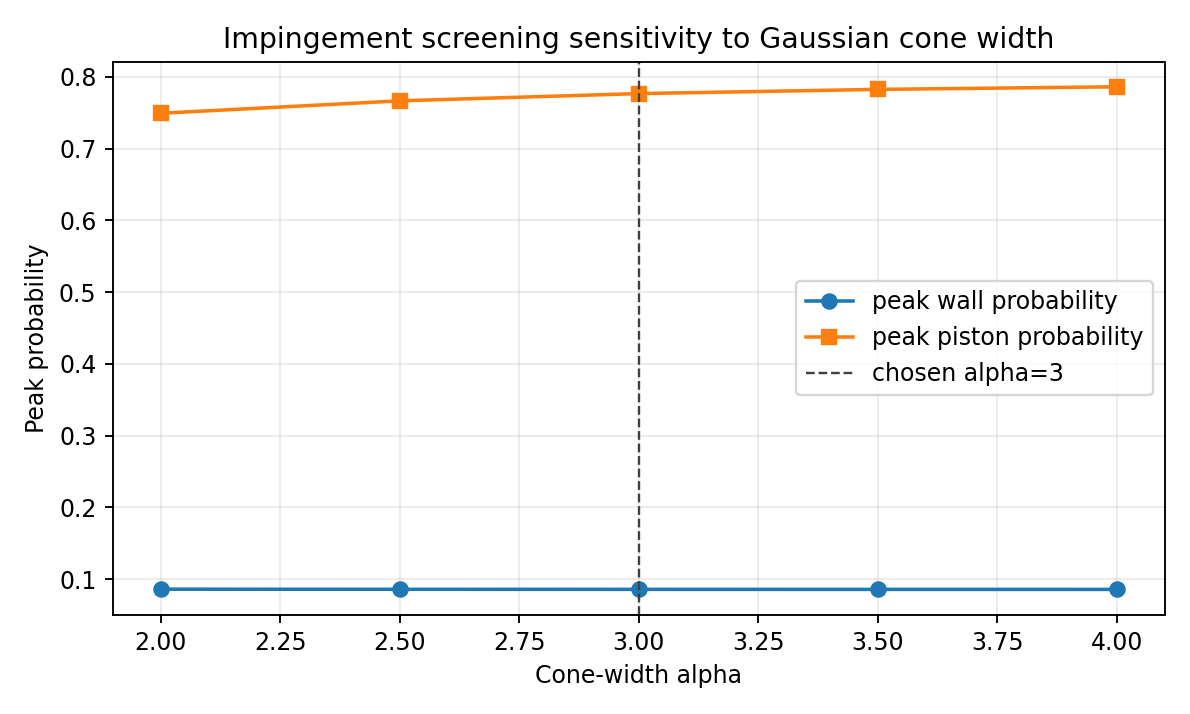
\includegraphics[width=0.82\linewidth]{../generated/current/alpha_sensitivity_figure.png}
\caption{横向 Gaussian 锥角宽度因子的生成式敏感性扫描。图中将选用的 \(3\sigma\) 解释与相邻 \(\alpha\) 取值并列，以显示筛查概率对这一建模约定的敏感程度。}
\label{fig:alpha-sensitivity-generated-zh}
\end{figure}

\textbf{活塞几何 dispatcher。}  原型给出三种可互换的冠面轮廓。默认 Design~A 采用分段圆弧构造，由外碗、内碗、顶岸、唇口和底部等半径参数拼接出盆状冠面；Design~B 则采用带切向约束的两圆弧碗形轮廓。Hermite 变体以\emph{五次 Hermite 样条}替代分段圆弧构造：冠面截面（径向、深度）由若干控制点定义，每个控制点携带位置和切向量，并在段间求得光滑过渡。在各节点处同时匹配位置、斜率与曲率，可在段间分界处实现 $C^{2}$ 连续，即冠面曲率无跳变。这一性质对 CNC 加工有实际意义——曲率不连续对应刀具加速度阶跃，会影响加工表面质量；同时也使碰撞积分栅格上的冠面 mask 更光滑，避免曲率突变在光栅化时产生锯齿。

该参数化方式也使系统性扫参更加方便：只需改变单个标量——例如碗底深度——整条冠面轮廓即可连续变形，样条自动将变化扩散到整段，无需重新求解任何约束方程。图~\ref{fig:hermite-crown}展示了四控制点基线冠面及其切向箭头（面板~a），以及对碗底深度进行七档扫描的结果（面板~b），直观说明了改变单一参数时冠面的连续光滑变形。三种设计均在与喷雾密度相同的画布网格上返回二值活塞 mask；最新默认图像使用的是 Design~A，因此图~\ref{fig:impingement-preview-zh}--\ref{fig:impingement-summary-zh} 中的黑色冠面并非 Hermite 扫参轮廓。

\begin{figure}[t]
\centering
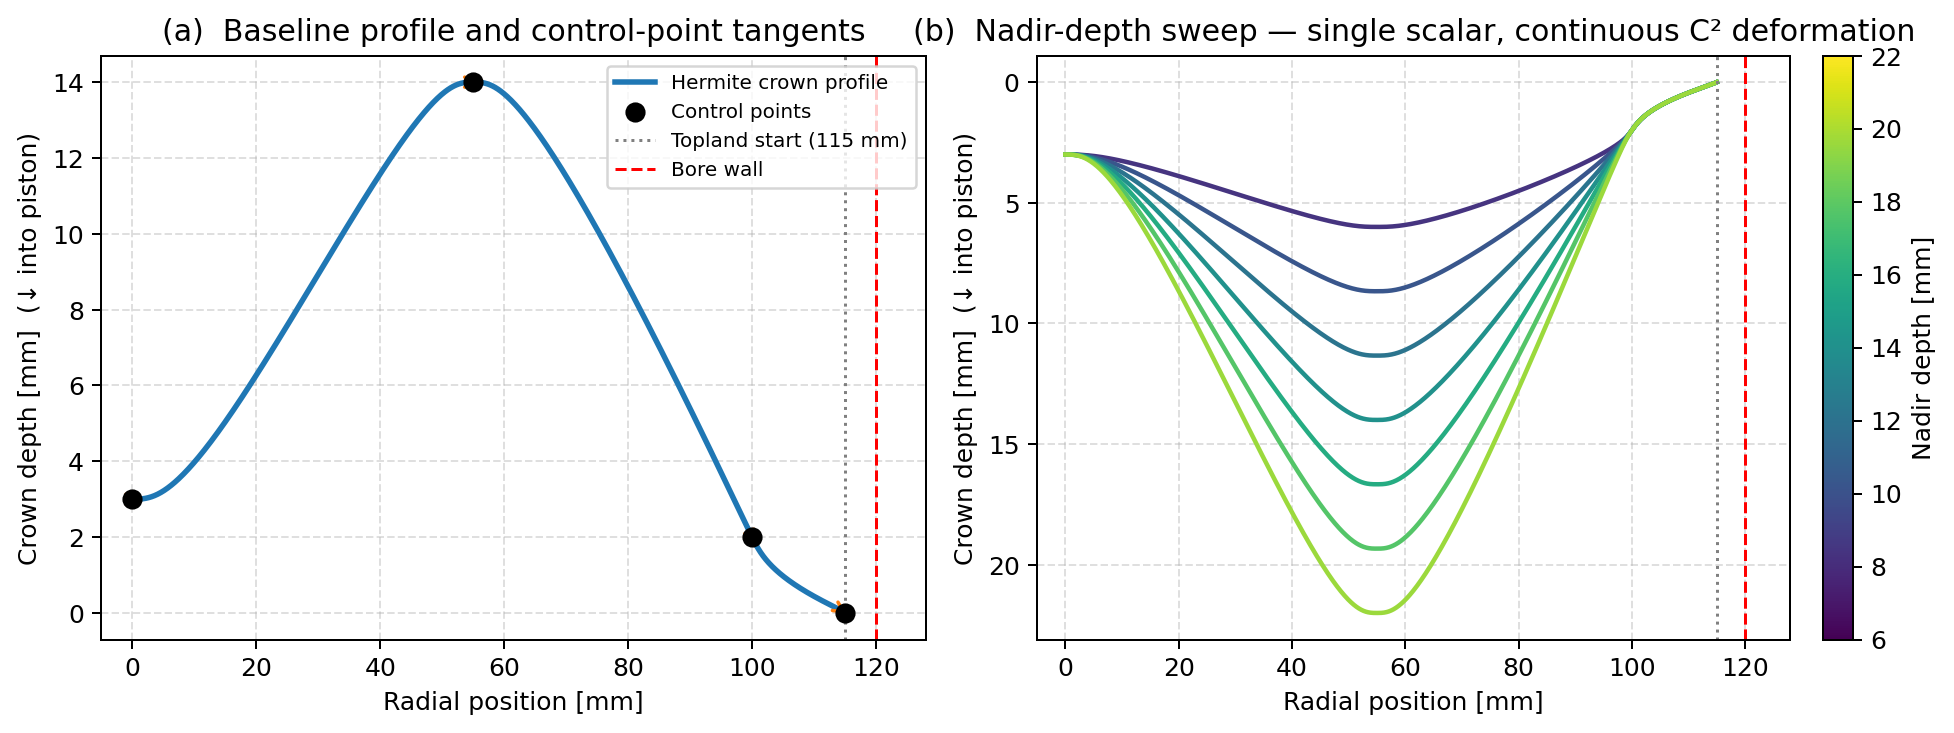
\includegraphics[width=0.96\linewidth]{images/hermite_crown_profile.png}
\caption{五次 Hermite 活塞冠面参数化。(a)~四控制点基线轮廓；实心圆点为控制点，橙色箭头为对应切向量。(b)~碗底深度从 \SI{6}{mm} 到 \SI{22}{mm} 的七档扫描：改变单个标量即可在保持各段 $C^{2}$ 连续的前提下，连续变形整条冠面轮廓。}
\label{fig:hermite-crown}
\end{figure}

\textbf{活塞运动学。}  活塞冠的轴向位置遵循简化的滑块--曲柄近似 \cite{HeywoodICE}
\[
h_{\mathrm{crown}}(t)=h_{0}-\tfrac{s}{2}\cos(\omega t+\varphi),\qquad \omega=\tfrac{2\pi\,\mathrm{RPM}}{60},
\]
其中实现中 \(t\) 以秒进入角速度项，GUI 时间轴以毫秒显示。该式为连杆比 $r/l\to 0$ 的简化形式，省略了高阶连杆修正项。相位 $\varphi$ 将参考事件置于 $t=0$。当前默认参数 $\mathrm{RPM}=250$、$s/2=\SI{55}{mm}$、$h_{0}=\SI{75}{mm}$、$\varphi=0$ 对应一个靠近上止点的短喷射窗口，在该窗口内冠面位移小于 \SI{1}{mm}，高阶修正可忽略。

\textbf{逐帧碰撞积分。}  瞬时碰撞概率与喷射窗口累积暴露量分别为
\[
P_{\mathrm{hit}}(t)=\iint p(x,y,t)\,\mathbf{1}_{\Omega_{\mathrm{piston}}(t)}(x,y)\,\mathrm{d}A,\qquad E=\int_{0}^{T} P_{\mathrm{hit}}(t)\,\mathrm{d}t,
\]
其中 \(\mathbf{1}_{\Omega_{\mathrm{piston}}(t)}\) 为活塞几何掩膜的瞬时二值指示函数；缸壁概率 \(P_{\mathrm{wall}}(t)\) 用同一 PDF 对 \(x\geq\SI{120}{mm}\) 的壁面 mask 积分得到。空间积分在画布网格上完成，累积暴露量在时间网格上用梯形求积。蒸馏学生的 onset 概率副输出保留在同一时间网格上，与 $P_{\mathrm{hit}}(t)$ 和 \(P_{\mathrm{wall}}(t)\) 并排绘制，使 SOI 附近的起始置信度与几何截获概率能够分开阅读。

\textbf{默认输出口径。}  最新 GUI artifact 的默认输入为 $d_n=\SI{0.34}{mm}$、喷油压力 \SI{2000}{bar}、腔压 \SI{15}{bar}、控制背压 \SI{4}{bar}、10 个 plume、喷射时长 \SI{800}{\micro s}、固定锥角 \(20^{\circ}\) 和倾角 \(20^{\circ}\)。在 0--\SI{5}{ms} 窗口内，绘图用的非负均值为 \(\mu_{+}(t)\in[\SI{1.70}{mm},\,\SI{112.95}{mm}]\)，轴向标准差为 \(\sigma_{\parallel}(t)\in[\SI{4.39}{mm},\,\SI{17.66}{mm}]\)，横向标准差为 \(\sigma_{\perp}(t)\in[\SI{0.50}{mm},\,\SI{6.64}{mm}]\)。Design~A 默认运行的活塞截获概率在 \(t=\SI{4.237}{ms}\) 达到峰值 \(P_{\mathrm{hit}}=0.7766\)，同帧缸壁截获概率为 \(P_{\mathrm{wall}}=0.0660\)；整个窗口的累积暴露量为 \(E=\SI{2.475}{ms}\)，最大缸壁概率为 \(0.0857\)。这些数值只说明端到端链路能够把穿深分布传播为可排序的时间分辨筛查分数；它们不应被解释为已验证的发动机内液滴碰壁概率。

\textbf{主张的边界。}  旋转 Gaussian 包络、解析锥角展宽与滑块--曲柄冠面模型都是工程化简化，并非在液滴尺度上求解的物理。该原型即文献综述所主张的那种概率性筛查 proxy，而非针对实验高速摄影或 CFD 碰撞场的已验证碰撞预测器。

本章所呈现的建模工作流——从清洗降阶目标，经分阶段异方差训练，到概率性碰壁评分——构成了本文的 surrogate 建模贡献。Stage~1、Stage~2、Stage~3 与物理及非参数基线在留出测试数据上的定量比较（包括覆盖率统计与留一喷嘴族压力测试）见第~5~章。当前章节建立了设计决策及其依据，结果则在后续章节中呈现。
